\documentclass[a4paper,12pt,twoside]{book}
\usepackage{graphicx}
\usepackage{natbib}
\graphicspath{ {figures/} }
\usepackage{array}
\usepackage{lipsum}
\usepackage{float}
\usepackage{siunitx}
\usepackage[T1]{fontenc}
\usepackage[utf8]{inputenc}
\usepackage[left=2.5cm,right=2.5cm,top=3cm,bottom=3cm]{geometry}
\tolerance=1
\emergencystretch=\maxdimen
\hyphenpenalty=10000
\hbadness=10000
\usepackage[belowskip=-10pt,aboveskip=10 pt]{caption}
\usepackage{setspace}
\def\bibfont{\footnotesize}
\doublespacing
\setlength{\intextsep}{20pt plus 2pt minus 2pt}
\setlength{\belowcaptionskip}{-15pt}

\usepackage{natbib}
\raggedbottom

\usepackage[french]{babel}
%\usepackage{lastpage}
\usepackage{fancyhdr}
\pagestyle{fancy}
\renewcommand{\headrulewidth}{2pt}
\renewcommand{\footrulewidth}{1pt}

\fancyhf{}
\renewcommand{\chaptermark}[1]{\markboth{\bsc{\chaptername~\thechapter{} :} #1}{}}
\renewcommand{\sectionmark}[1]{\markright{\thesection{} \ #1}}
\renewcommand{\headrulewidth}{0pt}
\lhead[\textsl{\leftmark}]{\textsl{\rightmark}}
\rhead[\textsl{\rightmark}]{\textsl{\leftmark}}
\cfoot[\thepage]{\thepage}



\renewcommand{\headrulewidth}{2pt}
\renewcommand{\footrulewidth}{1pt}
\begin{document}
	
	\frontmatter
	\input{Chaps/Dédicace.tex}
	\input{Chaps/Dédicace1.tex}
	
\chapter*{Remerciement}
Nous tenons à remercier nos professeurs de l'Institut Supérieur Des Etudes Technologiques De Béja pour leur support le long de notre parcours universitaire.

Nous tenons aussi à remercier notre encadrant professionnel et académique Mr.Aloui Radhouen pour son accueil et son accompagnement dans notre projet de fin d'études.

Finalement, nous remercions les membres honorés de Jury pour l'évaluation de notre travail.

	\tableofcontents
	\listoffigures
	\listoftables
	\mainmatter
	\markboth{INTRODUCTION}{}
	
\chapter*{Introduction générale}
La fusion de la composante logicielle (software) dans la composante matérielle (hardware) donne naissance généralement aux systèmes embarqués.
Selon les exigences, ces systèmes peuvent subir des adaptations matérielle ou logicielle. Il s'agit d'un système autonome qui doit réaliser son travail en tenant compte de plusieurs contraintes : sa taille, le temps d'exécution dont il dispose et l'énergie \cite{FUTURA}. Les systèmes embarqués sont très utilisés en aéronautique et dans l'industrie automobile. On les trouve également dans le domaine militaire à l'intérieur des missiles et bien évidemment dans l'agriculture, dans les distributeurs automatiques de billets, dans certains matériels médicaux, dans les imprimantes\ldots\  Depuis 2007, le secteur des systèmes embarqués a connu une croissance de $9,9\%$ de ses effectifs par an \cite{PierreAudoin2012} et une croissance qui devrait encore évoluer dans les prochaines années. Un système embarqué doit être capable d'exécuter des tâches en temps réel. Pour ce faire, il est équipé de capteurs, d'actionneurs et d'une interface. L'innovation des drones fait partie des systèmes embarqués les plus fréquents. 

Commençant par un aperçu sur l'historique du drone qui est développé par l'ingénieur et l'auteur anglais Archibald Low en 1916 pour les besoins de l'armée durant la première guerre mondiale \cite{STUDIOFLY}. 

De nos jours, cette innovation qui est nommée par les véhicules aériens sans pilote (UAV ou drones) est également un secteur en forte croissance, grâce aux avantages indéniables de la réduction des coûts par rapport aux hélicoptères, de l'élimination des risques de mise en danger de vies humaines dans certains cas, et de la rapidité de mise en œuvre \cite{AltiGator}. Les drones peuvent emporter une caméra, capable de retransmettre en temps réel ce qui se passe sur le terrain, une caméra infrarouge, détectant la chaleur (humaine, animale, d'un feu, d'un moteur, etc), un gyroscope permettant de stabiliser les mouvements du drone, améliorant le suivi d'une cible ou la qualité d'une image ainsi que la possibilité de former un ensemble de drones à intelligence collective, pour des applications civiles ou militaires. 

En outre, l'intelligence artificielle (l'IA) consiste à mettre en œuvre un certain nombre de techniques visant à permettre aux machines d'imiter une forme d'intelligence réelle. L'IA se retrouve implémentée dans plusieurs domaines d'application\cite{netactions} y compris surtout le domaine de l'agriculture. Elle assure le passage de l'agriculture traditionnelle vers l'agriculture de précision où la gestion de la production optimale. En effet, selon le dicionnaire \cite{leshorizons}, le principe de l'agriculture de précision consiste à utiliser les nouvelles technologies tels que l'intelligence artificielle, la robotique\ldots\ Cela pour augmenter les rendements d'une parcelle, d'optimiser le travail des agriculteurs et réduire la consommation d'énergie, d'eau et d'intrants.

Notre projet de fin d'études s'installe dans un cadre d'agriculture de précision dans laquelle on veut aider l'agriculteur à estimer sa production en combinant le système embarqué et l'intelligence artificielle. Le drone en tant qu'un système embarqué peut servir à résoudre certains problèmes urgents auxquels sont confrontés l'agriculture et l'environnement. L'utilisation de drones dans l'agriculture de précision permet de gérer la variabilité spatiale et temporelle pour améliorer les rendements économiques. Afin de s'organiser de manière appropriée, les agriculteurs ont besoin d'anticiper leur production notament que le manque d'une telle préditon de la récolte se traduit par des problèmes de distribution et de commercialisation.


Notre rapport est constitué de trois chapitres. Dans le premier, nous présenterons le cadre de projet y compris la problématique, l'objectif, la spécification des besoins et le cahier de charge. Le deuxième chapitre portera sur l'état de l'art de notre système qui sera expliqué en deux grandes parties. La première concerne le drone et la deuxième porte sur l'intelligence artificielle. Dans le dernier chapitre nous illustrerons la phase de la réalisation de notre projet.


	
	
	
	
	
	
	

	

	\chapter{Cadre du projet }
\newpage


\section{Introduction }
Dans ce chapitre, nous présenterons le contexte de notre projet en passant tout d'abord par sa  problématique et son objectif. Ensuite, nous détaillerons la méthodologie de gestion de ce projet ainsi que l'analyse des besoins de notre système. Finalement, nous clôturons ce chapitre par l'illustration des diagrammes SysML.

\section{Problématique }
Depuis des temps immémoriaux, l'agriculture était très importante dans la mesure où elle faisait partie intégrante de la vie humaine et demeure d'une grande importance économique et sociopolitique du fait de sa contribution à la réalisation des objectifs nationaux en matière de sécurité alimentaire, de création de revenus, d'emplois, d'équilibre régional et de gestion des ressources naturelles. Néanmoins ce secteur central a étalé une faiblesse importante mondiale et régionale de compétitivité sur les marchés nationaux et internationaux suite à un manque de la technique et de l'innovation qui reflète une faible production et l'absence de qualité des produits agricoles d'organisations professionnelles bien développée . Les agriculteurs doivent constamment faire des miracles pour trouver des solutions à de nouveaux problèmes. Les défis à relever à l'avenir peuvent être très différents des problèmes rencontrés aujourd'hui. Pour cette raison-là, l'agriculture a connu de nombreuses crises vue qu'elle utilise les mêmes moyens sans innover de nouvelles technologies ni augmenter sa productivité.

Ces dernières années, le monde a été confronté à une baisse importante de la production agricole. Par exemple, au Brésil, le premier producteur d'oranges dans le monde avec plus de 19 millions de tonnes d'où proviennent plus de la moitié des fruits utilisés pour fabriquer les jus consommés à travers le monde. D'après les estimations du département américain de l'Agriculture (Usda), la situation est particulièrement critique vu que la production d'oranges risque d'être la plus faible depuis plus de vingt ans. En Tunisie, la production d'agrumes de la campagne 2017/2018 a fortement chuté à 38,2 \%, soit 346 000 tonnes \cite{onagri2017/2018}.

En plus, récemment à cause de cette crise sanitaire dûe au covid19, le secteur agricole rencontre d'autres problèmes et d'autres challenges. Il a perturbé le fonctionnement de l'agriculture et du système alimentaire dans son processus de production menant au centre de consommation. En raison des restrictions, il n'y a moins de travailleurs et des ouvriers dans de nombreux secteurs et domaines, ce qui peut facilement affecter la production et les économies mondiales et régionales. Le confinement des pays et la fermeture des frontières ont une forte incidence sur la rapidité et la flexibilité du modèle agricole. Il y'a donc moins d'innovations alternatives ce qui peut refléter un ralentissement de la production agricole.
\section{Objectif }
L'objectif de notre projet de fin d'études est d'utiliser les nouvelles technologies pour améliorer les performances économiques et environnementales des productions agricoles. Afin de s'organiser de manière appropriée, les agriculteurs ont besoin d'anticiper leur production. Mais le comptage des fruits est une tâche qui prend beaucoup de temps. Notre projet nommé « AGRIDrone » est consacré à optimiser ce temps perdu par le développement d'un système automatisé intégré dans un drone pour le comptage des oranges sur l'arbre. 


Ce système va mettre au point une méthode de travail plus efficace et bien précis qui utilise l'intelligence artificielle pour permettre aux fournisseurs de produits agricoles d'optimiser leurs récoltes et de planifier leurs ventes sur le marché. La technologie des drones pourrait aider les agriculteurs du monde entier à surveiller la croissance de leurs cultures, lutter contre les nuisibles, et bien plus encore. Grâce à la caméra et aux capteurs embarqués, le drone peut mesurer de nombreux indicateurs de l'état et des besoins de la plante. En fait, notre système fournit des informations plus précises et une variété de données.

Bien que le prélèvement ait été exécuté manuellement, les informations recueillies par le drone permet aux agriculteurs d'identifier les zones à traiter, de déterminer l'intervention la plus appropriée et de réduire la quantité de traitement utilisée. Tout cela sera facile et nous fera gagner de temps non négligeable avec cette nouvelle innovation.



\section[Methodologie]{Méthodologie de gestion de projet }
Cette méthodologie nous permet d'analyser l'environnement de notre projet, d'appliquer des méthodes techniques et d'évaluer l'opportunité jusqu'à l'achèvement de notre travail.
\subsection{Choix de méthodologie }
Afin d'assurer le bon déroulement des différentes étapes dans notre projet, nous avons choisi la méthode Agile Scrum pour gérer notre travail, concevoir et développer nos systèmes pour des raisons claires. Ce processus  s'inscrit parfaitement dans la décomposition de notre projet qui s'appuie sur les avantages suivants :
\begin{itemize}
	\item Plus de flexibilité et de réactivité
	\item Traduire et organiser le projet de façon simple, transparente et pragmatique
\end{itemize}

\subsection{Présentation de la méthodologie scrum }
La méthodologie Scrum nous a aidé dans la gestion de notre travail en planifiant les tâches à réaliser durant notre projet. D'abord, nous préparons ces tâches. Puis, nous assistons à une réunion pendant 15 minutes afin de les sélectionner et démarrer un sprint. Ensuite, nous classifions dans un tableau agile les activités selon l'avancement de chacune (à faire, en cours, sprint review, sprint retrospective et fini). Finalement, nous fermons le sprint pour passer à un autre.
Il existe trois rôles principaux intervenant dans la méthode agile scrum:
\subsubsection{Product owner }
C'est la personne ayant la responsabilité de produire et de maintenir à jour le carnet de produit. Elle détermine les priorités et prend les décisions d'orientation du projet.
\subsubsection{Scrum master  }
Celui qui s’assure que les principes et valeurs du scrum sont
respectées et veille au bon déroulement et avancement du projet. De plus, il facilite la communication au sein de l’équipe ainsi qu'il cherche à améliorer la productivité et le savoir-faire de son équipe.
\subsubsection{L'équipe développement  }
Constituée généralement de 2 à 10 développeurs. Elle regroupe tous les rôles habituellement nécessaires à un projet tels que l'architecte, le concepteur, le développeur, le testeur,... Elle est « auto-organisée » et reste inchangée pendant toute la durée du sprint.

La figure ci-dessous présente le déroulement de la gestion de projet par Scrum \cite{Crochet}.

\begin{figure} [H]
	\begin{center}
		\centering
		\hspace*{-0.5cm}
		\fbox{\includegraphics[width=0.67\linewidth]{Images/Méthode Scrum}}
	\end{center}
	\caption{Agile Scrum}
\end{figure}
\section{Analyse des besoins }	
L'analyse des besoins est une des premières techniques de gestion de projet à mettre en oeuvre.

Cette partie sera utilisée pour jeter les bases de la collecte des besoins du système avant d'être réalisée.
Dans le but de préciser les besoins des utilisateurs de notre système, nous présenterons les besoins fonctionnels ainsi que les besoins non fonctionnels.

\subsection{Les besoins fonctionnels}
Notre projet consiste à développer un drone qui doit survoler la parcelle tout en inspectant les arbres afin de détecter pour chaque arbre les oranges présentes.

Parmi les différents besoins fonctionnels de notre système, nous citons:
\begin{itemize}
	\item Le paramétrage du contrôleur de vol 
	\item  La configuration de la radiocommande 
	\item Le contrôle de l'AGRIDrone
	\item La génération des rapports
\end{itemize} 

En plus, les besoins fonctionnels et les attentes vis-à-vis notre AGRIDrone varient d'un acteur à un autre. Pour celà, nous allons détailler le rôle de chaque acteur en se basant sur des diagrammes de cas d'utilisation \ref{Cas d'utilisation}.

\subsection{Les besoins non fonctionnels}
Après avoir cité les besoins fonctionnels, nous présentons
les besoins non fonctionnels de drone qui sont liés aux contraintes dont il faut tenir compte pour appliquer une solution adéquate et qui ont été définis tels que:
\begin{itemize}
	\item \textbf{La stabilité :}
	
	
	Dans le cadre de ce travail, le drone devra être stable, l'AGRIDrone doit être robuste en terme de repositionnement automatique aprés une perturbation.	
	
	\item \textbf{L'extensibilitè : }
	
	
	L'AGRIDrone doit permettre des nouvelles fonctionnalités.
	
	\item \textbf{La portée : } 
	
	
	On doit pouvoir contrôler le drone jusqu'à 500m
	
	
	\item \textbf{La maintenabilité : }  
	
	Subir à une intervention de maintenance en terme de modifications et corrections des erreurs.
	\end {itemize}
	\section{Diagramme d'exigence }
	Après avoir étudié attentivement les besoins de  notre système, nous avons effectué sa modélisation à travers le diagramme d'exigence permettant de décrire graphiquement les capacités à réaliser et les contraintes qui doivent être dépassées.
	
	Une exigence comporte : 
	\begin{itemize}
		\item Un intitulé 
		
		\item Un texte descriptif 
		
		\item Un identifiant unique
	\end{itemize}
	
	\begin{figure}[H] 
		\begin{center} 
			\centering
			\hspace*{-1.3cm} \fbox{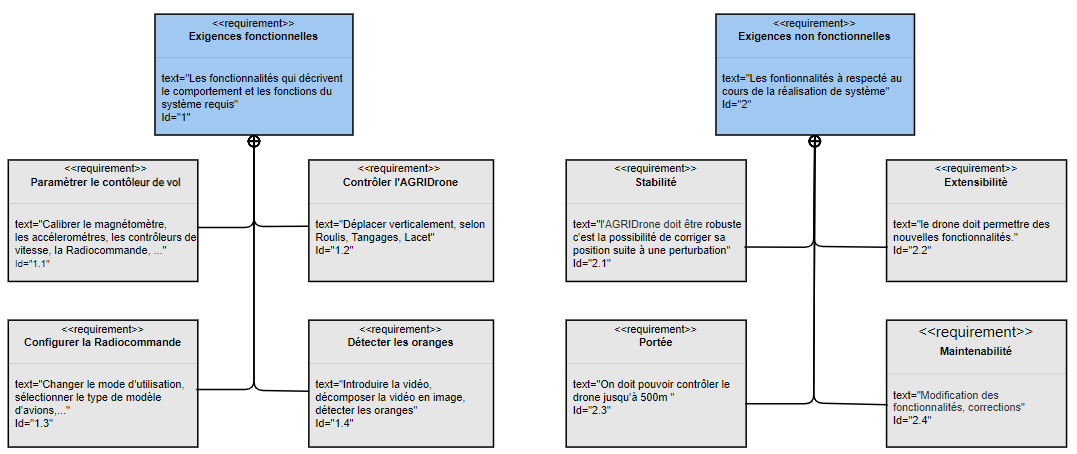
\includegraphics[width=1.26\linewidth]{Images/Diagramme d'exigence}}
			
			\caption{Diagramme d'exigence}
		\end{center}
		\end {figure}
		
		\section[D.des cas d'utilisation]{Diagrammes des cas d'utilisation }\label{Cas d'utilisation}
		
		Cette structure est bien adaptée pour décrire de manière claire les fonctions et les objectifs les plus importants d'un système. C'est pour cette raison que l'élaboration d'un diagramme de cas d'utilisation est souvent l'une des premières étapes lors de la conception de système ou de la planification de nouveaux processus métier. Cela permet de visualiser facilement et clairement quels cas d'utilisation doivent être pris en compte dans la conception pour que les acteurs atteignent les objectifs escomptés. 
		
		Nous illustrons dans la suite les principaux diagrammes de cas d'utilisation.
		\subsection{Cas d'utilisation global }
		Nous décrivons en tant qu'utilisateurs ce diagramme  qui donne un aperçu global sur le rôle de chaque acteur afin de comprendre l'idée générale du projet.
		
		
		\begin {figure} [H]
		\begin{center}
			\centering
			\hspace*{-0.8cm}\fbox{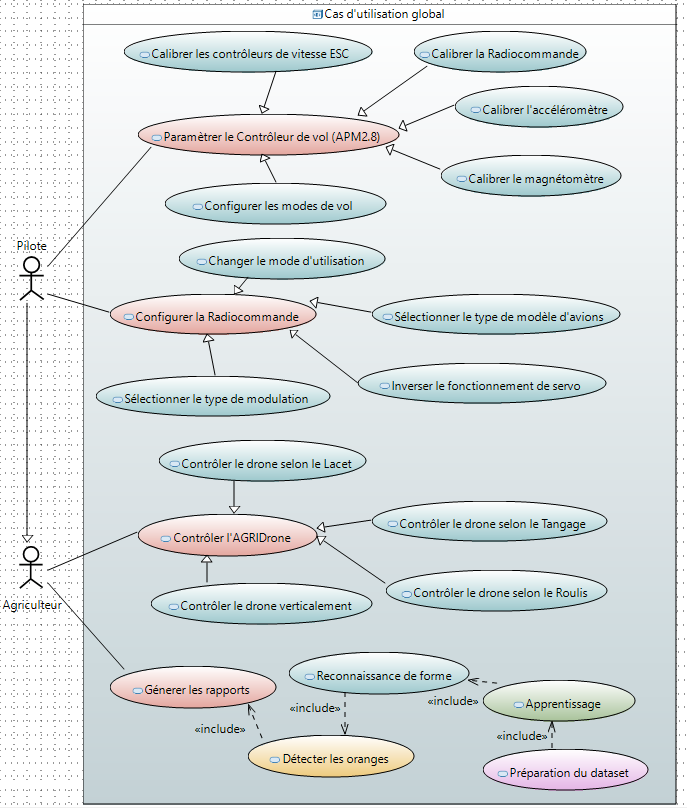
\includegraphics[width=1.17\linewidth]{Images/Diagramme de cas d'utilisation globale}}
		\end{center}
		\caption{Diagramme de cas d'utilisation global}
		\end {figure}
		
		Ci-dessous nous exposons quelques cas d'utilisation afin de mieux comprendre les caractéristiques contenues dans chaque cas.
		
		
		\subsection{Cas d'utilisation du Pilote}
		Nous montrons à travers la figure \ref{fig:D.P} le diagramme de cas d'utilisation du pilote qui permet de déterminer les principales fonctions qu'il doit effectuer. À savoir, en paramétrant le contôleur de vol, cet acteur a la possibilité de calibrer les contrôleurs de vitesses, la radiocommande, l'accéléromètre, le magnétomètre et régler les modes de vol. La deuxième tâche consiste à configurer la radiocommande d'où la possibilité de changer le mode d'utilisation, sélectionner le type de modèle d'avions, inverser les fonctionnements du servos et sélectionner le type de modulation. Le pilote doit aussi contrôler l'AGRIDrone en le déplaçant verticalement, selon le lacet, le tanguage et le roulis.
		\begin {figure}[H] 
		\begin{center} 
			\centering
			\hspace*{-0.1cm}		\fbox{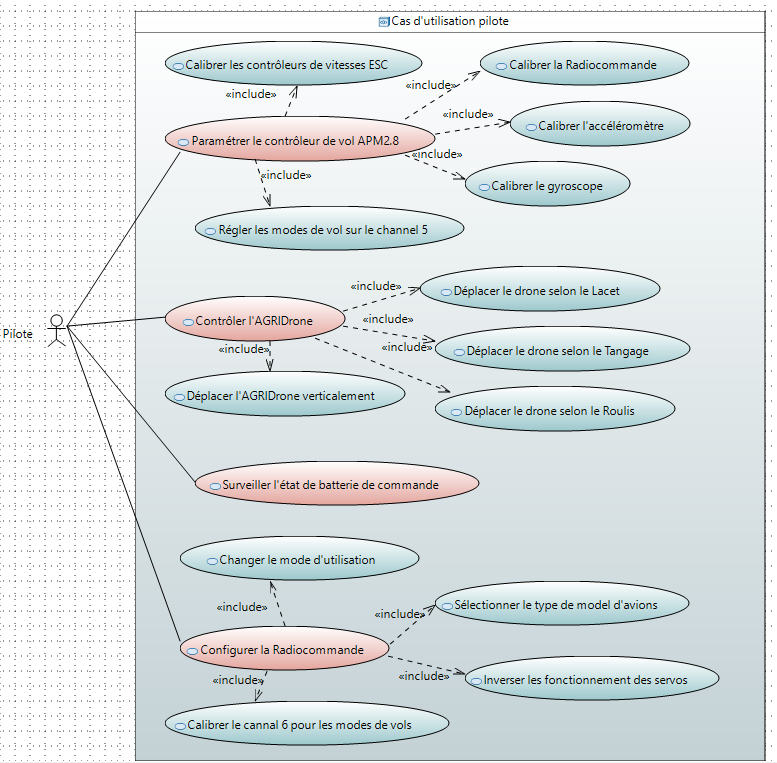
\includegraphics[width=1\linewidth]{Images/Diagramme de cas d'utilisation pilote}}
		\end{center}
		
		\caption{\label{fig:D.P}Diagramme de cas d'utilasation pilote}
		\end {figure}
		
		
		\subsection{Cas d'utilisation de l'agriculteur }
		La figure \ref{fig:D.A} décrit le cas d'utilisation de l'agriculteur qui peut contrôler l'AGRIDrone avec les mêmes procédures que suit le pilote et générer les rapports après avoir détecter les oranges. Cette opération à son tour se produit à condition que la reconnaissance de forme s'établit. 
		\begin{figure}[H] 
			\begin{center} 
				\centering
				\hspace*{-0.7cm}	\fbox{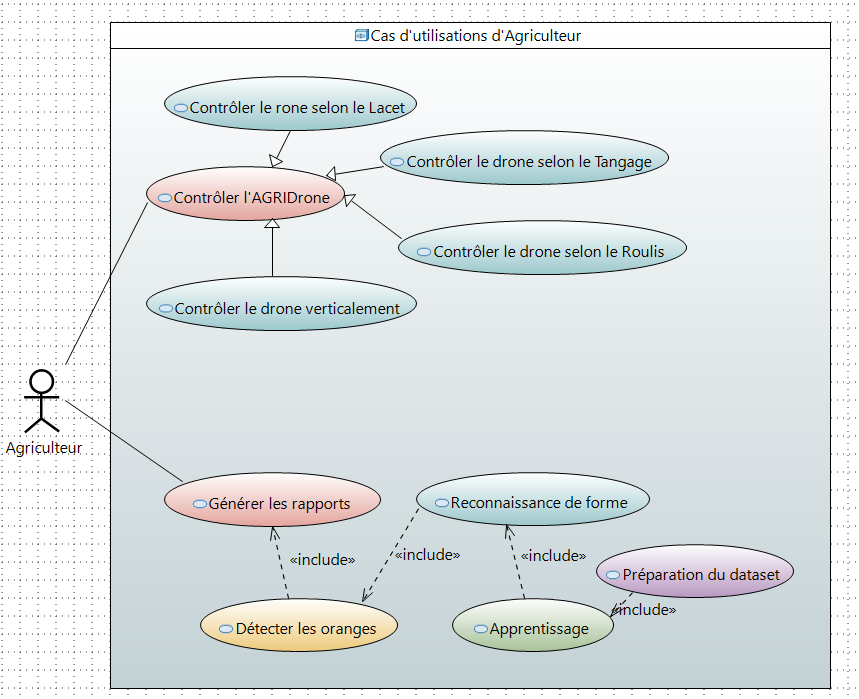
\includegraphics[width=1\linewidth]{Images/Diagramme de cas d'utilisation agriculture}}
			\end{center}
			
			\caption{\label{fig:D.A}Diagramme de cas d'utilisation d'agriculteur}	
			
			\end {figure}
			
			\section*{Conclusion}
			Le long de ce chapitre, nous avons exposé la problématique à partir de laquelle nous avons créé l'objectif de notre projet et nous avons montré la phase de la méthodologie de travail, de la spécification des besoins et de la conception des diagrammes SysML.
			
			Dans le chapitre suivant, nous présentons l'état de l'art de notre système.
			



	
\chapter{Etat de l'art }

\clearpage
\section*{Introduction}
Ce chapitre portera en premier lieu sur le drone avec ses différents types et mouvements ainsi que sa stabilisation. En second lieu, nous détaillerons la partie qui concerne l'intelligence artificielle et nous passerons au concept de la détection des fruits. 
 
\section{Drone}	
Les drones sont des aéronefs sans équipage dont le pilotage est automatique ou télécommandé. Leur masse varie de quelques grammes à plusieurs tonnes\cite{Wikipideaa}. Il sont moins chers et plus simples à mettre en œuvre qu'un avion. Ils sont aussi plus discrets et leur perte est moins grave que celle d'un appareil avec son pilote.

Dans cette section, nous allons étudier les principaux types de drone ainsi que les multirotors que nous avons choisi. En plus, nous allons passer aux différents domaines d'application du quadrirotor, ses mouvements, sa stabilisation et les applications d'un quadrirotor basés sur la vision artificielle.   	
\subsection{Les types des drones}
Il existe plusieurs types de drones, nous avons mis l'accent sur deux types: aile fixe et multirotor.
	
	\subsubsection{Aile fixe }
	L'avion à voile fixe est capable de voler en utilisant des ailes qui génèrent une élévation causée par la vitesse avant du véhicule et la forme des ailes\cite{educalingo}.
	
	
	\begin{figure}[H] 
	\begin{center} 
		\centering

 \fbox{	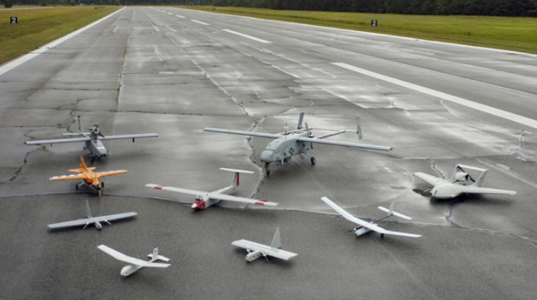
\includegraphics[width=0.6\linewidth]{Images/Ailes fixed}}
		
	\end{center}
	
	\caption{Ailes fixes Drones}
	\end{figure}
	\subsubsection{Multi-rotors}
	C'est le type de drone qui possède plusieurs rotors sur son corps. Cette caractéristique lui offre la possibilité de rester en position unique pendant une longue période. En plus, ces drones sont très pratiques pour diverses utilisations.
	\begin {figure}[H] 
	\begin{center} 
		\centering
			\pagestyle{fancy}
		\hspace*{-0.7cm}
	\fbox{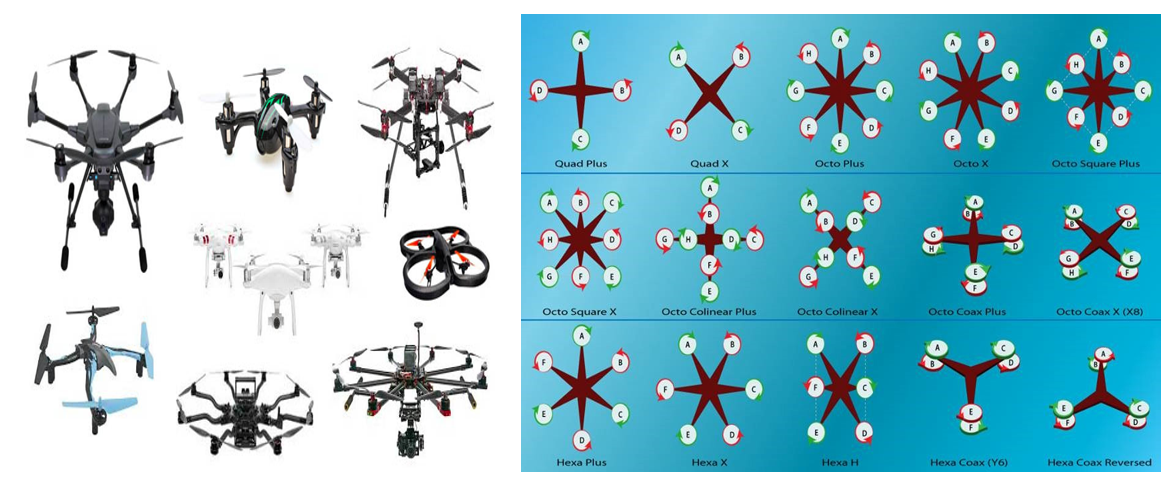
\includegraphics[width=1.1\linewidth]{Images/Types des multirotor}}
		
	\end{center}
	
	\caption{Types des multirotors}
	\end{figure}
	\subsubsection{Comparaison entre un drone aile fixe  et un drone multirotors}
	Après avoir étudié chaque type de drone, nous avons effectué une étude comparative entre eux selon plusieurs critères : vitesse, niveau de contrôle, capacité de charge, endurance et atterissage/décollage.
	
	Nous remarquons à travers ce tableau que les drones à voilure fixe sont plus rapides que les drones à voilure tournante. Ils sont difficiles à contrôller, supportent une faible charge et nécessitent des grandes surfaces pour l'atterissage et le décollage.
    Vu que notre situation nécessite une vitesse adapté à notre système de détection des oranges, nous avons choisi le quadrirotor qui est facile à contrôler, supporte une charge importante et pratique dans les petites surfaces.      
	\begin{table}[H]
		\begin{center}
			\vspace{0.5cm}\caption{Comparaison entre un drone aile fixe  et un drone multirotors }
			\begin{tabular}{|c|c|c|}
				\hline
				\centering
				& 
				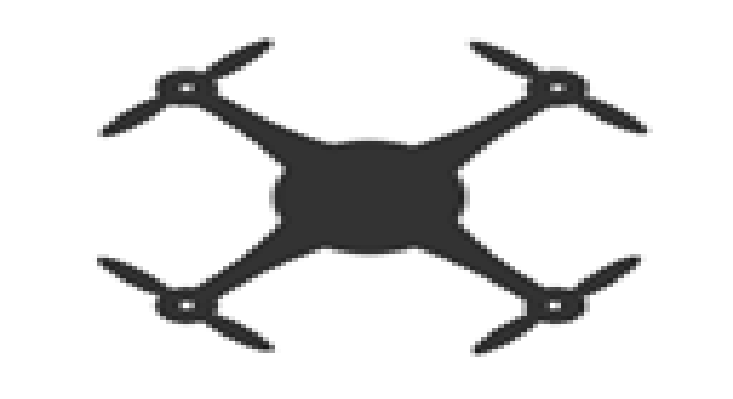
\includegraphics[scale=0.2]{Images/Quadrirotor}
				&
				
\includegraphics[scale=0.2]{Images/Ailed fixed}\\
				
				\hline
				Vitesse & 70 Km /h - 250 Km /h & 100 Km /h-700 Km /h  \\
				\hline
				Contrôle	& facile &	difficile \\
				\hline
				Capacité de charge &	grande charge &	petite charge \\
				\hline
				Endurance &	15min-60min & 1h-12heures \\
				\hline
				Atterrissage et décollage &	petites surfaces &	grandes surfaces \\
				\hline
			\end{tabular}
		\end{center}
	\end{table}	
\subsection{Définition du quadrirotor}
C'est un aéronef à voilure tournante à quatre rotors qui sont généralement placés à l'extrémité de la croix. Pour empêcher l'appareil de tourner sur lui-même autour de son axe de lacet, il faut que deux hélices tournent dans un sens et les deux autres dans le sens inverse\cite{Wikipidea}. Pour pouvoir diriger l'appareil, il faut placer chaque paire d'hélices qui tournent dans le même sens aux extrémités opposées de la branche transversale.
	\begin{figure}[H] 
	\begin{center} 
		\centering
\fbox{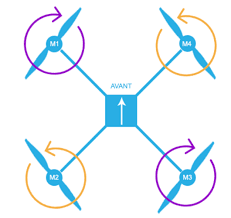
\includegraphics[width=0.42\linewidth]{Images/Sens de rotation des moteurs}}	
	\end{center}
	\caption{Sens de rotation des moteurs }
	\end{figure}
	\subsection{Histoire des quadrirotors}
	Le premier quadrirotor à décoller du sol est le gyroplane Breguet-Richet, développé par la société Breguet en 1907. Il ne décolle qu'à une hauteur de 60 cm et quatre hommes maintiennent la structure\cite{Wikipidea}. 
	\begin{figure}[H] 
	\begin{center} 
		\centering
	\fbox{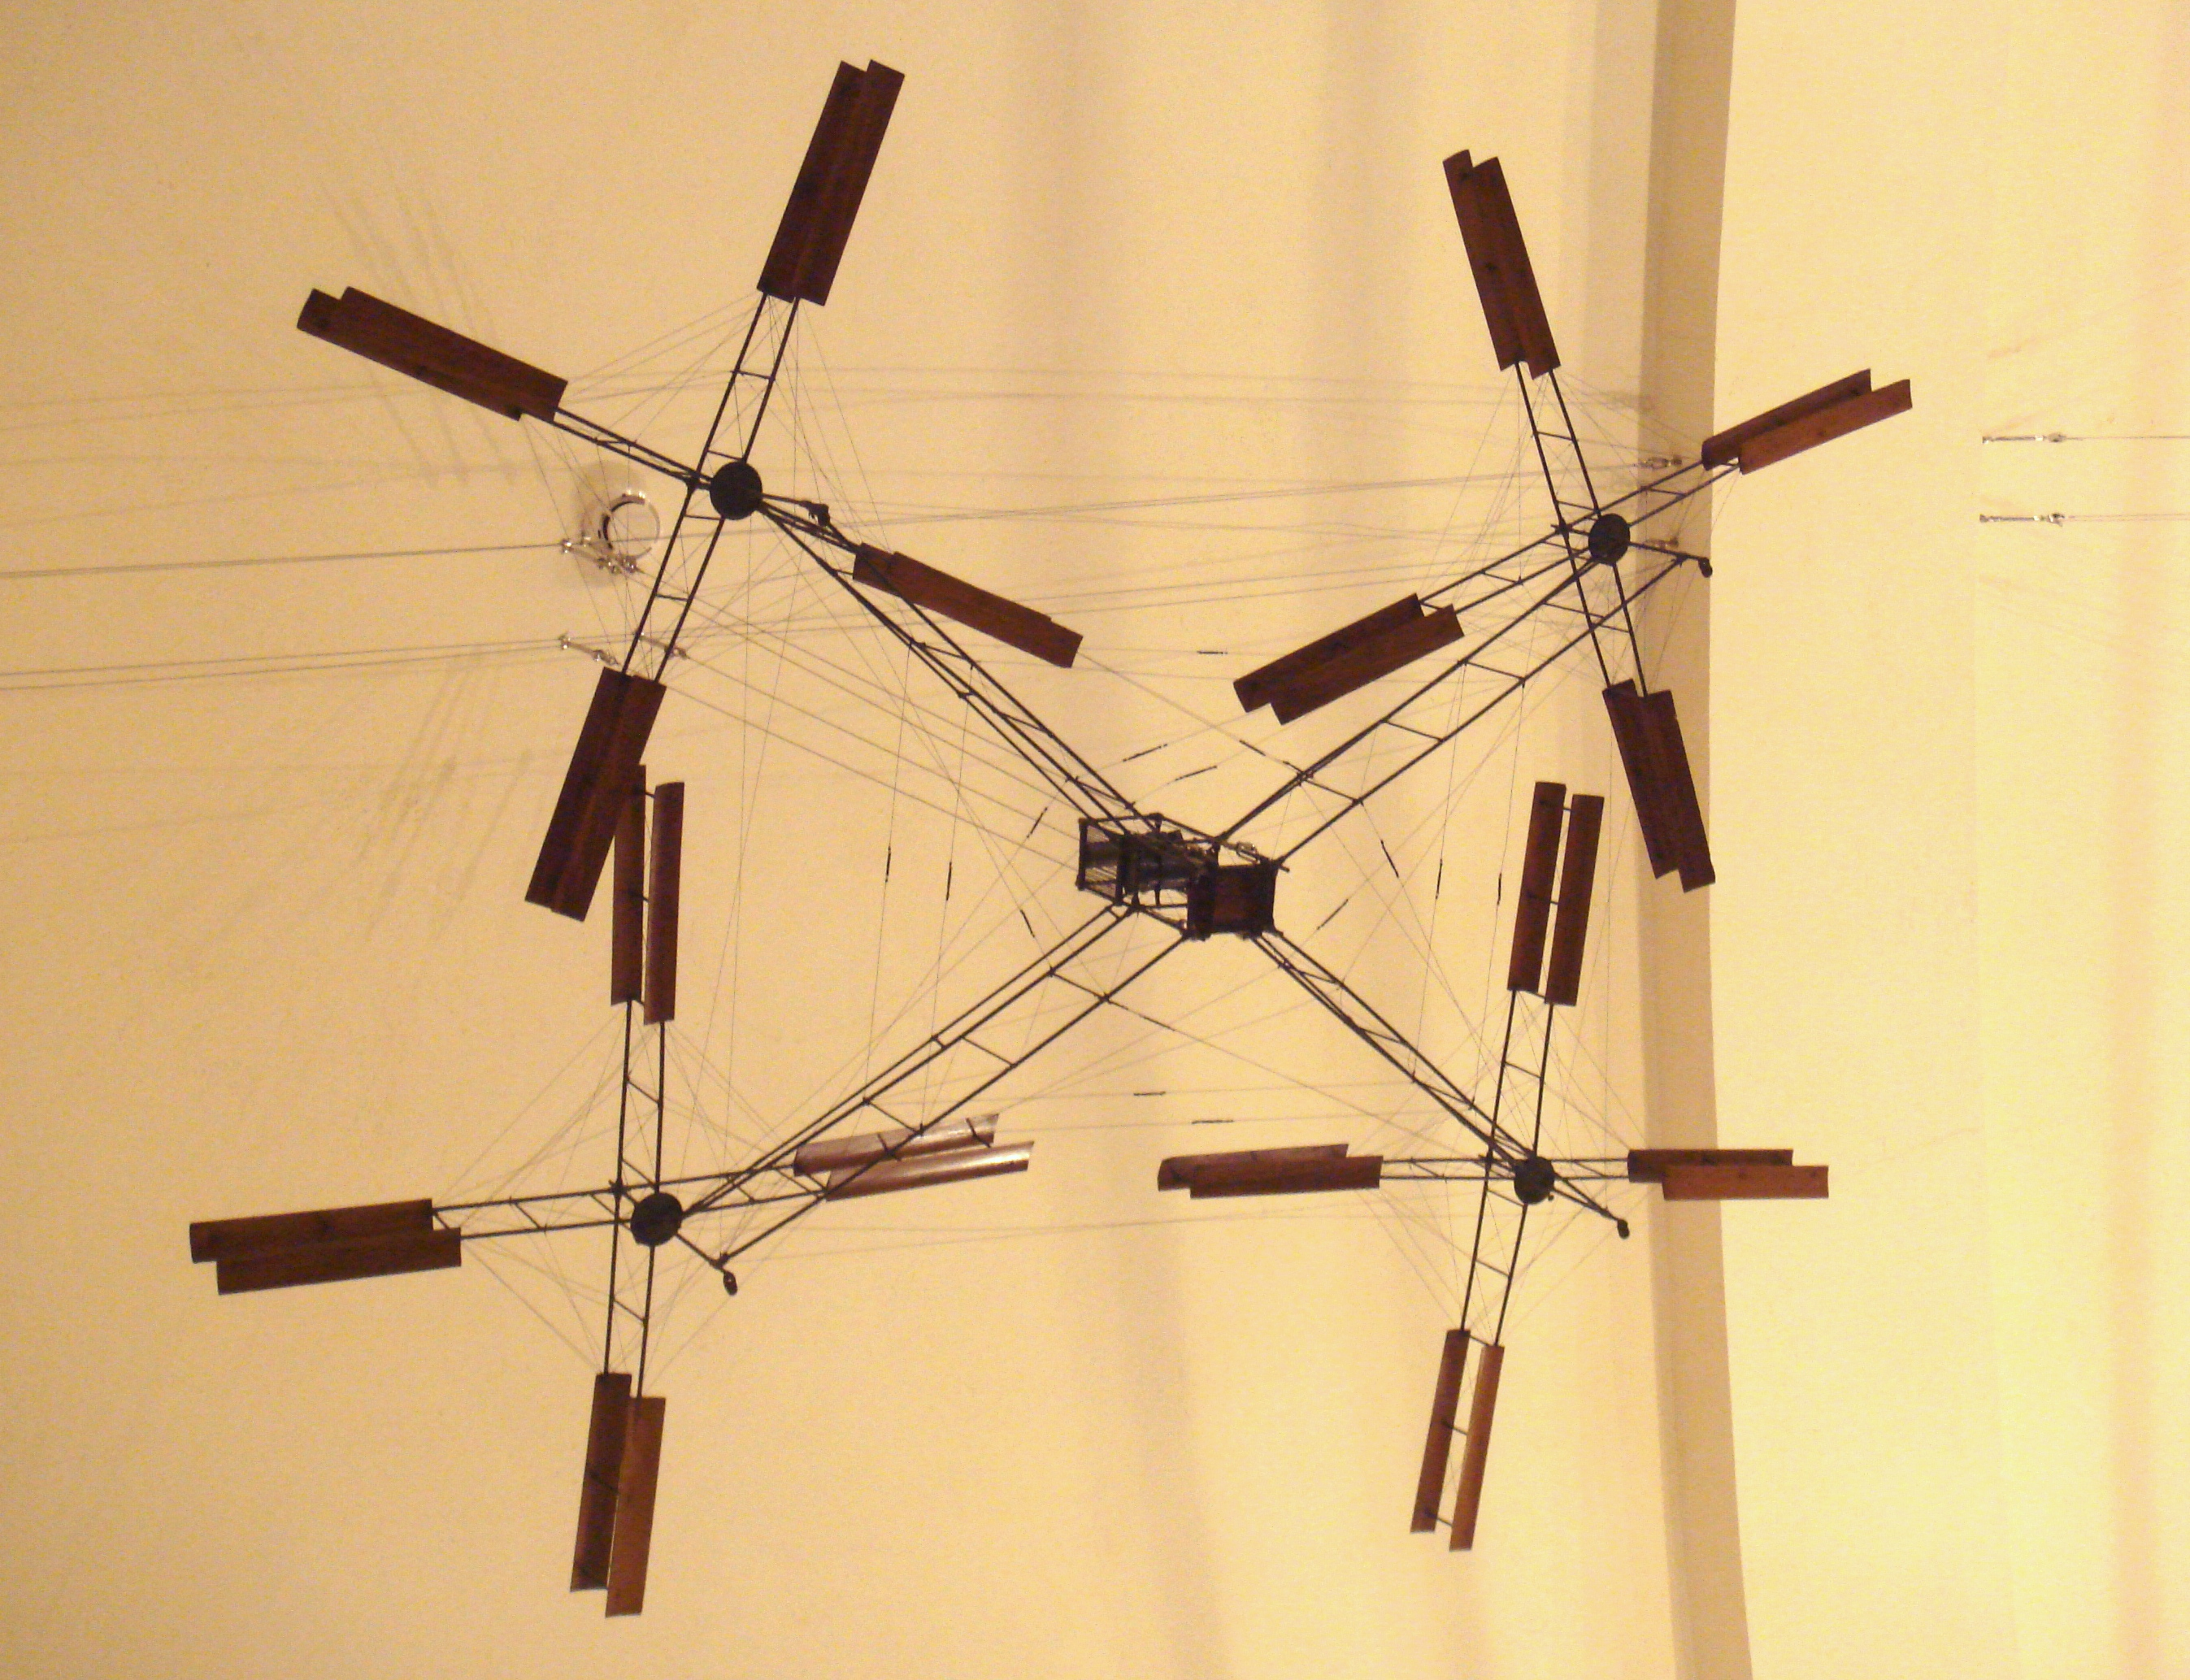
\includegraphics[width=0.6\linewidth]{Images/Breguet_Gyroplane_1907}}
		
	\end{center}
	\caption{Gyroplane }
	\end{figure}

	\subsection{Les domaines d'applications du quadrirotor}
	 
	Le quadrirotor est de plus en plus répandu dans le secteur professionnel grâce à son apport d'information, son autonomie et sa rapidité. Parmi ses différents domaines d'applications, nous citons: 
	
	\begin{itemize}
		
		\item [$\bullet$]Le militaire et la protection civile
		\item [$\bullet$]La sécurité et la surveillance
		\item [$\bullet$]L'agriculture
		\item [$\bullet$]Le journalisme
		\item [$\bullet$]Le FPV racing
		
	\end{itemize}
	\newpage
	\subsection{Mouvements du quadrirotor}
	Les mouvements de base du quadrirotor sont réalisés en variant la vitesse de chaque rotor et en changeant la poussée produite. Ces mouvements sont couplés, ce qui signifie que le quadrirotor ne peut pas faire de translation sans réaliser un mouvement de roulis ou de tangage \cite{WikiMemoires}.
	
	Nous présentons ci-dessous les mouvements effectués par le quadrirotor:		
	\begin{itemize}
		\item[$\bullet$] \textbf{Mouvement vertical}
		\item[$\bullet$] \textbf{Mouvement de roulis} 
		\item[$\bullet$] \textbf{Mouvement de tangage}
		\item[$\bullet$] \textbf {Mouvement de lacet}
	\end{itemize}
	\begin{figure} [H]
	\begin{center}
		\centering
	\fbox{	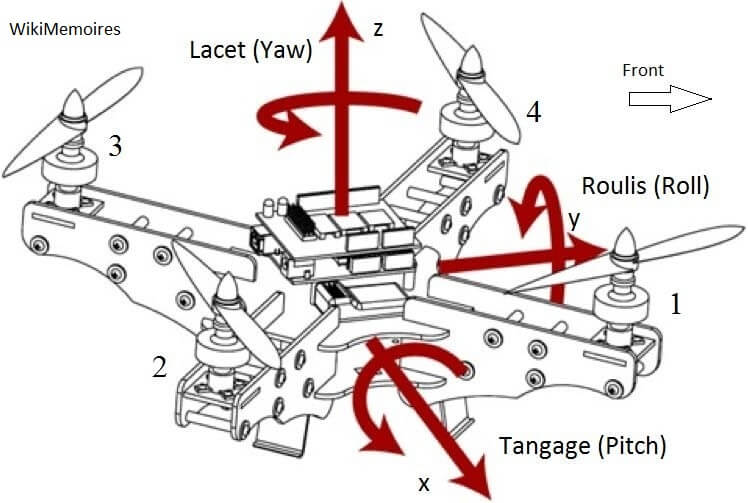
\includegraphics[width=0.7\linewidth]{Images/Les mouvements du drones}}
	\end{center}
	\caption{Les mouvements du drones}
	\end{figure}

	
	\subsubsection{Mouvement vertical}
	Pour monter, nous augmentons la vitesse des moteurs simultanément, tous les moteurs tournent au même régime et inversement pour descendre. Cette manipulation s'effectue à travers la commande des gaz.
	\begin{figure} [H]
	\begin{center}
		\centering
	\fbox{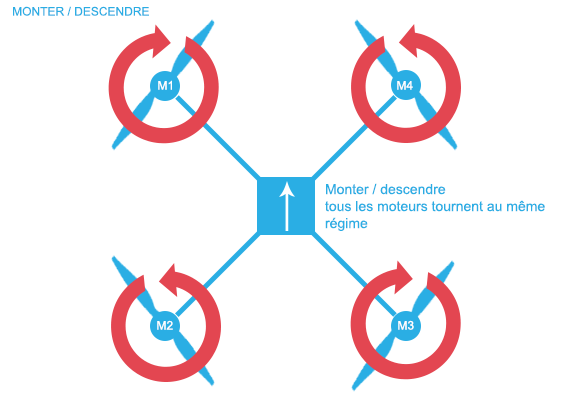
\includegraphics[width=0.6\linewidth]{Images/Mouvement vertical}}
	\end{center}
	\caption{Mouvement vertical}
	\end{figure}

	\subsubsection{Mouvement de roulis}
	Pour incliner vers la gauche, nous diminuons les moteurs de gauche et augmentons ceux de droite. Inversement pour incliner vers la droite. Cette action s'appelle le roulis.
	\begin{figure} [H]
	\begin{center}
	
	\fbox{	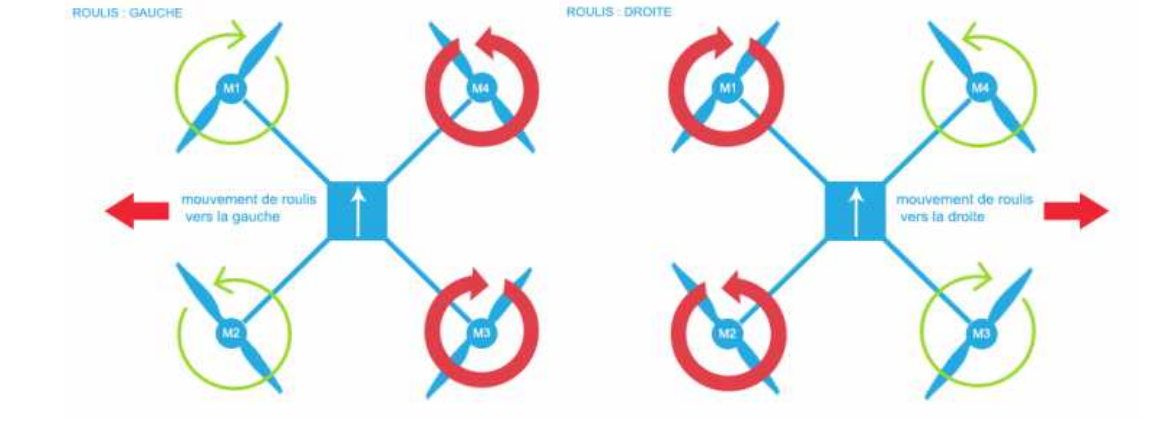
\includegraphics[width=1\linewidth]{Images/Mouvement de roulis}}
		\caption{Mouvement de roulis}
	\end{center}
	\end{figure}
	\subsubsection{Mouvement de tanguage}
	Pour avancer, nous diminuons la vitesse des moteurs avant et augmentons la vitesse des moteurs arrière et inversement pour reculer. C'est le tangage.
	
	
	\begin{figure}[H] 
	\begin{center}
		\centering
		\fbox{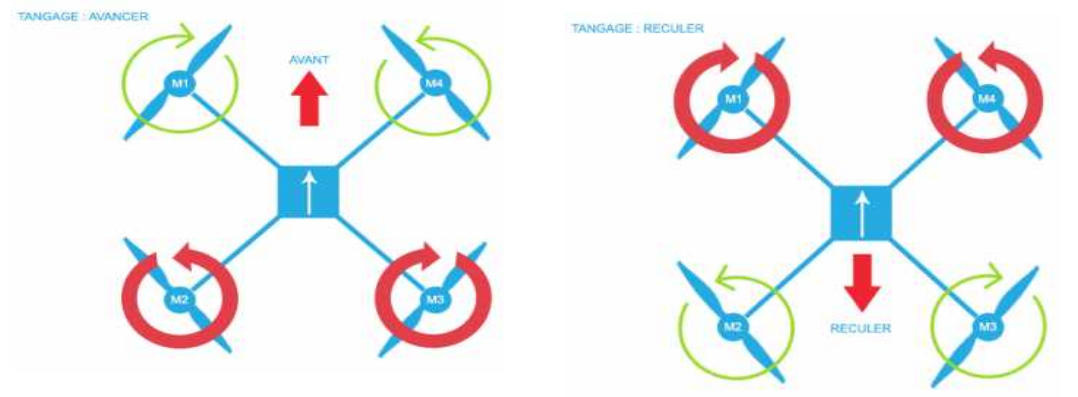
\includegraphics[width=1\linewidth]{Images/Mouvement de tanguage}}
	\end{center}
	\caption{Mouvement de tanguage}
	\end{figure}
	
	\subsubsection{Mouvement de lacet}
	Pour un mouvement de rotation, nous augmentons la vitesse d'une paire de moteurs sur le même axe et inversement. Ceci est un mouvement de lacet.
	\begin{figure} [H]
	\begin{center}
\fbox{	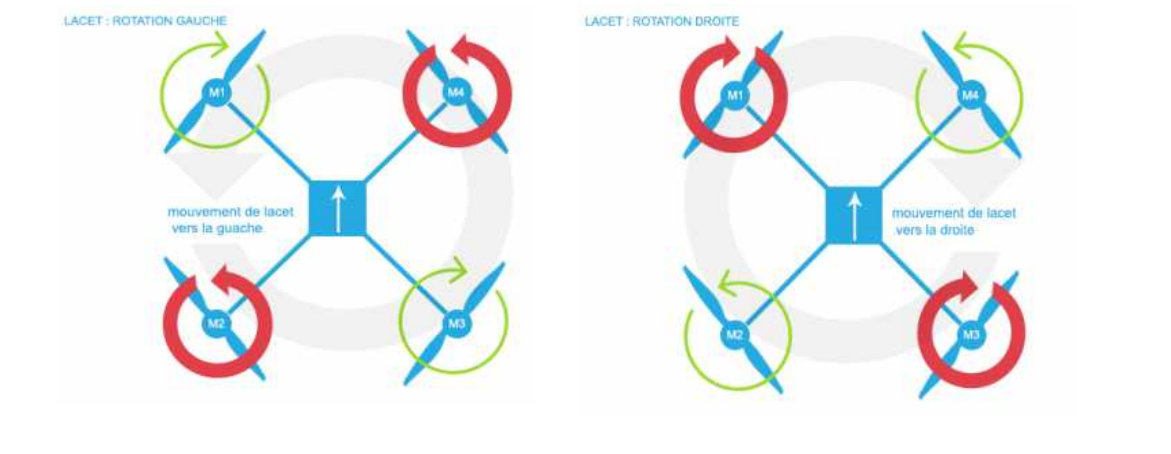
\includegraphics[width=1\linewidth]{Images/Mouvement de lacet}}
	\end{center}
	\caption{Mouvement de lacet}	
\end{figure}
\subsection {Stabilisation du quadrirotor}
Pour assurer la stabilisation du quadrirotor, nous avons trouvé que la solution adéquate à cette opération est le régulateur "PID" qui représente un système de contrôle permettant d’améliorer les performances d'un asservissement\cite{Wikipideab}.
	\begin{figure}[H] 
	\begin{center}
		\centering
		\fbox{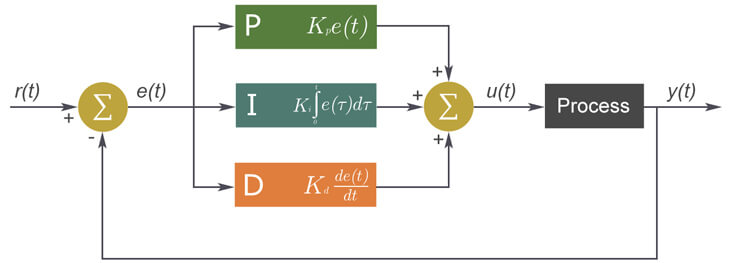
\includegraphics[width=0.7\linewidth]{Images/asservi PID}}
	\end{center}
	\caption{Système asservi PID}
\end{figure}

Nous définissons l'action PID en détaillant chacune de ses parties.
\subsubsection {Action PID} 
Le régulateur PID combine les trois actions vues précédemment et permet ainsi d'avoir de bonnes performances aussi bien en vitesse, en stabilité et en précision. L'expression d’un régulateur PID \cite{WikiMemoiresa}est donné comme suit :

 $ c(t)=K_p\times \epsilon(t) + K_i\int\epsilon(t)dt+K_d\frac{d\epsilon(t)}{dt}$


Ainsi ce régulateur permet d'atteindre les objectifs fixés en termes de vitesse de stabilité et de
précision et ce en trouvant la configuration optimale des valeurs des différents gains $K_p $, $ K_i$ et $ K_d$.
\subsubsection {Action proportionnelle}
L'effet de l’action proportionnelle consiste à amplifier l'erreur d’un gain constant afin que le
système réagisse plus rapidement aux changements de consigne. Cette action proportionnelle est
représentée par l'équation suivante:

$ c(t) = K_p\times \epsilon(t) $


Plus la valeur de $K_p$ est grande plus la réponse est rapide mais au détriment d'une détérioration
de la stabilité du système allant jusqu'à l'instabilité pour de grandes valeurs.
\subsubsection  {Action intégrale}
L'action intégrale a pour but de réduire voire d'éliminer l'erreur statique en régime permanent. Pour réaliser cela le régulateur intègre l'erreur par rapport au temps et multiplie le résultat par une
constante $K_i$ comme ci-dessous :

$c(t) $ =$ K_i\times\int \epsilon(t) dt$


Plus la valeur de $K_i$ est grande plus l'erreur statique sera vite corrigée mais nous perdons un peu
en stabilité et il y a un risque de dépassement.

\subsubsection  {Action dérivée}
Pour obtenir une action dérivée, nous multiplions la dérivée de l'erreur par un coefficient $K_d$.
Cette action permet d'éliminer le dépassement de la réponse et d'améliorer la stabilité du système. Sa relation est donnée comme suit :

$ c(t)  = K_d\times\frac{d\epsilon(t)}{dt}$


Plus la valeur de Kd est grande plus le dépassement est atténué mais si elle est trop grande le
système est ralenti jusqu'à risquer de devenir instable pour de très grandes valeurs.
\subsection{Applications de quadrirotors basées sur la vision artificielle}
L'emploi de l'intelligence artificielle sur les quadrirotors est une innovation qui a réalisé plusieurs succès dans les différents domaines d'applications. Cette procédure facilite notre mode de vie vu qu'elle nous permet de gagner du temps et d'effectuer des tâches complexes.

Nous pouvons distinguer quatre principaux types d'applications:   
\begin{itemize}
	\item[$\bullet$]Évitement d'obstacles 
	\item[$\bullet$] Suivi de cible
	\item[$\bullet$] Atterrissage de drones 
	\item[$\bullet$] Détection d'objets 
\end{itemize}
\begin{figure}[H]
	\centering
	\begin{minipage}{0.49\textwidth}
		\fbox{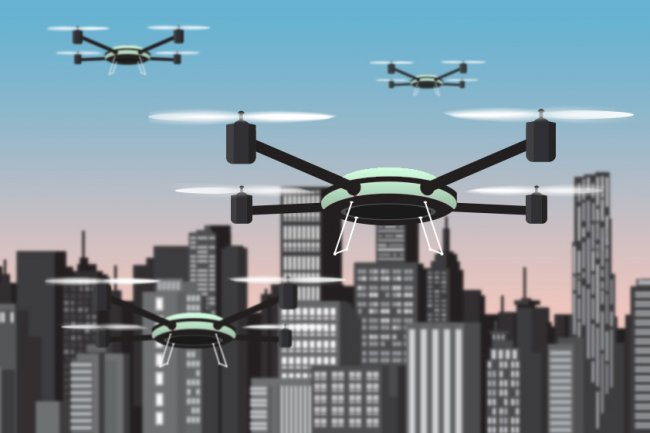
\includegraphics[width=0.8\linewidth]{Images/Evitement d'obstacles}}
		\caption{Évitement d'obstacles}
		
	\end{minipage}
	\begin{minipage}{0.49\textwidth}
		\fbox{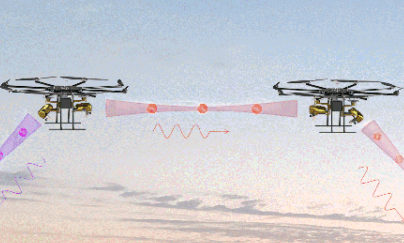
\includegraphics[width=0.9\linewidth]{Images/Quadrirotor mener par un autre}}
		\caption{Suivi de cible}
	\end{minipage}
\end{figure}
\begin{figure}[H]
	\begin{minipage}{0.49\textwidth}
\fbox{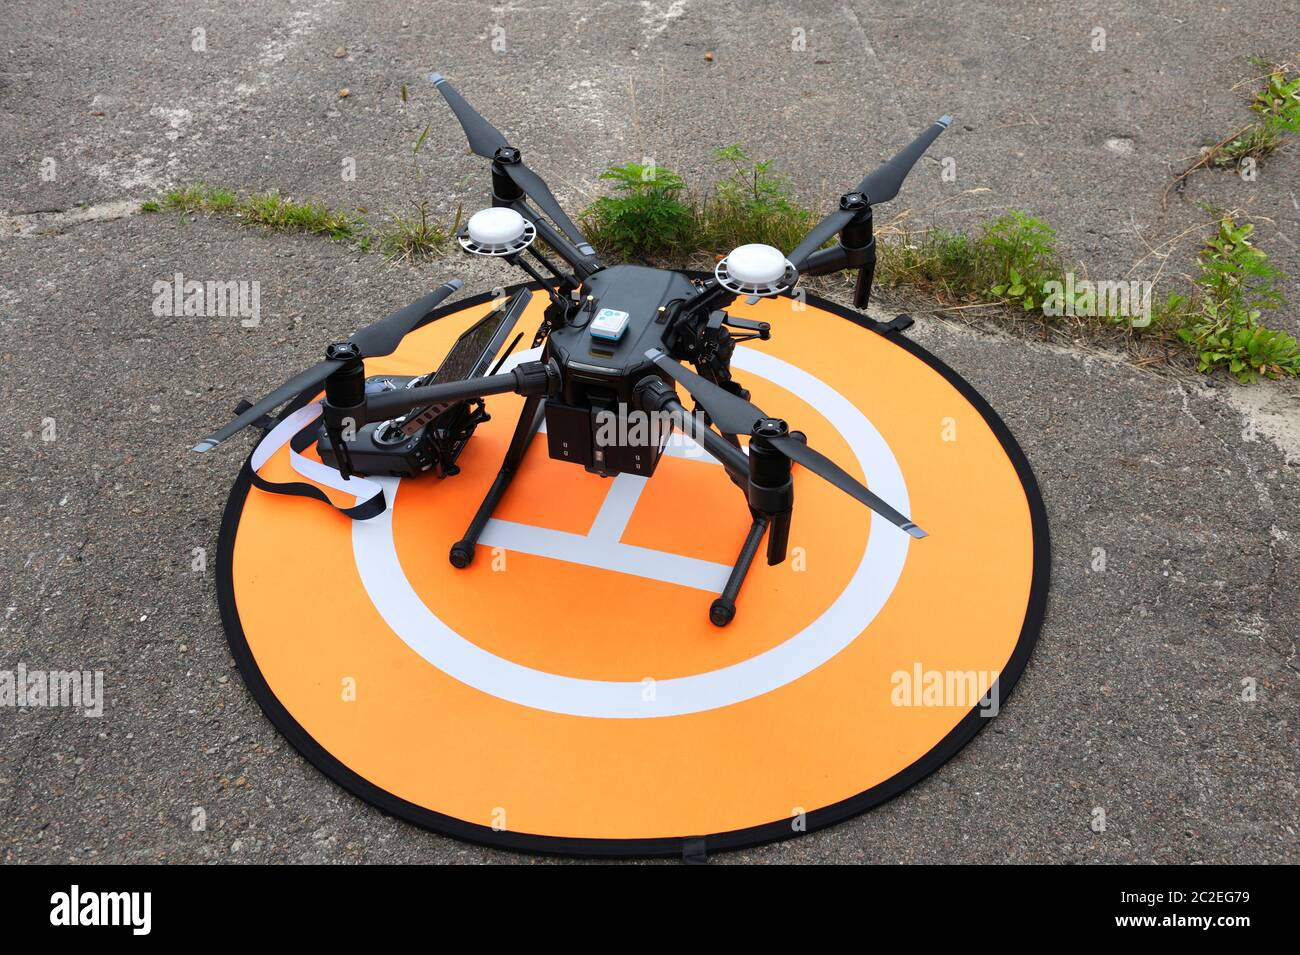
\includegraphics[width=0.8\linewidth]{Images/Atterissage de quadrirotor}}
		\caption{Atterrissage }
	
	\end{minipage}
	\begin{minipage}{0.49\textwidth}
		\fbox{\includegraphics[width=0.8\linewidth]{Images/Détection d'objet}}
		\caption{Détection d'objets }
		
	\end{minipage}
\end{figure}
\section{Intelligence artificielle}
Le but de l'intelligence artificielle est de concevoir des systèmes capables de reproduire le comportement de l'humain dans ses activités de raisonnement \cite{PowerPoint}. C'est pour cela, nous avons employé cette technologie dans notre système puisqu'elle le rend autonome, c'est à dire il raisonne d'une façon fiable et précise. 
Durant cette partie, nous allons expliquer en premier lieu le concept général de la détection des fruits, nous détaillerons ensuite le déroulement de la détection des oranges. En second lieu nous allons décrire le réseau de neurones puis la détection des objets par encadrement. Nous allons finir cette section par la description de l'outil Yolo. 

\subsection{Détection des fruits}
La détection et la classification des fruits restent difficiles en raison de la forme, de la couleur et de la texture des différentes espèces de fruits. En étudiant l'impact de la vision par notre système sur cette opération, nous avons souligné que jusqu'aujourd'hui, la méthode d'apprentissage en profondeur(Deep learning) est la plus pratique pour la détection et la classification des fruits. C'est pour cette raison que nous avons décidé de l'employer dans notre projet. Puisque la couleur orange est attractive ainsi qu'on la trouve dans plusieurs catégories d'oranges, nous avons choisi de travailler spécifiquement sur la détection des oranges.
\subsection{Détection des oranges et comptage}
Notre approche consiste en plusieurs étapes. D'abord, nous détectons les oranges sur des images acquises dans les vergers par une des méthodes de détection d’objets. Ensuite, nous améliorons ces résultats en caractérisant les pixels acquis sur les oranges. Enfin, nous estimons une position  dans l’image plus précise pour les oranges détectées, ainsi que leur taille moyenne.
	\begin{figure} [H]
	\begin{center}
		\fbox{\includegraphics[width=0.4\linewidth]{Images/Détection des oranges}}
		\caption{Détection des oranges}
	\end{center}
\end{figure}

\subsection{Réseau de neurones}
Ce réseau est un système informatique s'inspirant du fonctionnement du cerveau humain. Il existe le réseau de neurones récurrents et le réseau de neurones convolutifs \cite{Lebigdata}.

Afin de détecter et catégoriser les objets souhaités facilement, nous avons choisi de travailler avec le réseau de neurones à convolutions qui doit passer par une phase d’apprentissage avant d’être utilisé comme détecteur. Le but de cette dernière est de lui apprendre à reconnaitre une ou plusieurs classes d’objets. Pour cela, nous lui fournissons un ensemble d’images contenant les objets en question que nous souhaitons encadrer et classifier.
\subsection{Détection d'objet par encadrement}
Après avoir classifié les objets à travers le réseau de neurones, il est nécessaire d'employer la détection d'objet par encadrement qui consiste à dessiner un cadre de délimitation autour de chaque objet dans l’image sous forme d'un rectangle.
\subsection{Détection en temps réel}
C'est un système d'où le comportement se base sur l'exactitude des traitements effectués et surtout le temps requis pour produire ses résultats. Ceci nous permet de gagner en terme de temps et de vitesse d'exécution.
\subsection{Yolo}
Dans un premier temps, étant donné que le modèle de détection doit être à la fois précis et rapide dans son exécution, les outils de détection en temps réel constitue la première approche de ce projet. Selon l’état de l’art, le choix de l’outil YOLO était le plus adéquat à nos besoins. 

Ce dernier découpe l’image en une grille de taille S × S. Puis de façon simultanée, il réalise d’une part la prédiction des objets dans l’image et d’autre part, détermine la classe de l’objet \cite{towardsdatascience.}, comme montré sur la figure \ref{fig:A.Y}
\begin{figure} [H]
	\begin{center}
		\fbox{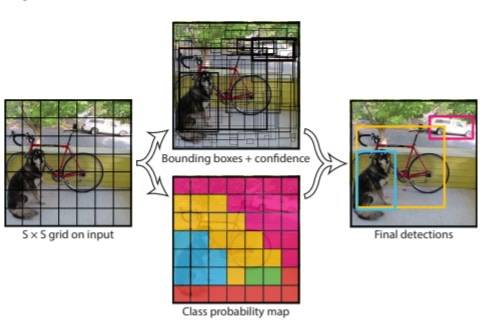
\includegraphics[width=0.8\linewidth]{Images/Architecture Yolo}}
		\caption{\label{fig:A.Y}Architecture de Yolo}
	\end{center}
\end{figure}
\section*{Conclusion}
Durant ce chapitre, nous avons donné les 
généralités sur le drone. Nous avons présenté et expliqué le fonctionnement du quadrirotor ainsi que l'implémentation de l'intelligence artificielle pour la détection des oranges.

Le dernier chapitre sera consacré pour la réalisation de notre projet.

	

\chapter{Réalisation du projet}
\clearpage
\section*{Introduction}

Dans ce chapitre nous présenterons les différentes étapes de réalisation de notre projet en exposant le matériel utilisé et son diagramme de définition de bloc. Par la suite, nous expliquerons les logiciels avec lesquels nous avons travaillé. Finalement, nous détaillerons la configuration et la calibration de l'APM2.8 et la radiocommande, ainsi que les étapes que nous avons effectué pour résoudre le problème rencontré dans notre travail. 

\section{Matériels utilisés}
Lors de notre réalisation, nous avons utilisé plusieurs composants que nous présentons ci-dessous.
\subsection{Châssis}
Le châssis représente le corps principal de notre quadrirotor. Il comprend quatre bras de forme "X". Ses caractéristiques à prendre en compte sont le poids, qui est lié aux matériaux utilisés et sa résistance au choc. Plus le châssis est léger, plus nous conservons de la puissance.

Pour éliminer les vibrations du moteur et pour obtenir les meilleures performances aérodynamique, nous avons choisis d’utiliser un châssis professionnel "le DJI F450". Il est fabriqué en PA66 et 30GF qui offre une meilleur résistance aux dommages sur les atterrissages durs \cite{smartcube}, son assemblage est simple et rapide. Les 4 bras sont vissés entre la plaque inférieure et la plaque supérieure. Notre châssis a une envergure de 450 mm et pèse 272 grammes.
Cette structure permet d'accueillir toute l'électronique : ESCs, moteurs, contrôleur de vol. En plus, nous pouvons grâce au PCB intégré dans la plaque inférieure souder les pôles du contrôleur de vitesse (+/-) et la batterie. La propulsion recommandée repose sur le châssis qui est capable de supporter un poids total en vol situé entre 800 et 1600 grammes maximum a l'aide des moteurs 2212 \cite{studiosport}.

\begin{figure} [H]
	\begin{center}
		\centering
		\fbox{\includegraphics[width=0.3\linewidth]{Images/Châssis DJI F450}}
	\end{center}
	\caption{Châssis DJI F450}
\end{figure}

\subsection{Moteur Brushless}
Notre drone nécessite l'utilisation de moteurs ayant une très grande vitesse en considérant leur poids qui doit être léger. Ceci nous oblige d'utiliser des moteurs brushless \underline{A2212} qui sont des moteurs à courant continu, n'utilisent pas de balais collecteurs car les bobines sont alimentées directement au stator et que les aimants sont placés sur le rotor \cite{Cube}. Afin d'obtenir un vol stable et un couple de moteurs important, nous avons choisi ces composants possédant 930KV. A savoir, KV représente la constante de vitesse qui est le nombre de tours par minutes divisé par les volts KV=RPM/U. Par exemple, lorsque nous attribuons à un moteur une tension de 10V, celui-ci tournera à 9300 tr/min. 
\begin{figure} [H]
	\begin{center}
		\centering
		\fbox{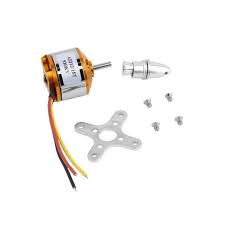
\includegraphics[width=0.3\linewidth]{Images/Moteur Brushless}}
	\end{center}
	\caption{Moteur Brushless}
\end{figure}
\subsection{Contrôleur de vitesse électronique (ESC)}
Concernant l'étage de puissance, nous avons opté pour un contrôleur de vitesse ESC (Electronic Speed Controller) pour contrôller l'énergie délivrée aux moteurs brushless  grâce à la tension de sortie modulable d’une carte programmable. Ces appareils reçoivent des signaux PWM (Pulse Modulation Width)\cite{altidrone}, cette commande est alors traduite en une alimentation triphasée avec une fréquence particulière qui va faire tourner les moteurs. Vu que le contrôleur de vitesse doit être supérieur au courant maximum du moteur qui est de 10A, nous avons choisi un courant de 30A. 
\begin{figure} [H]
	\begin{center}
		\centering
		\fbox{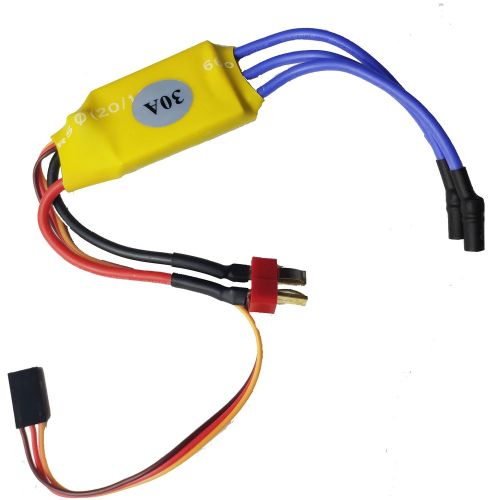
\includegraphics[width=0.3\linewidth]{Images/Contrôleur de vitesse électronique (ESC)}}
	\end{center}
	\caption{Contrôleur de vitesse électronique (ESC)}
\end{figure}

\subsection{Batterie}
L'alimentation électrique de notre système est une procédure très importante pour le fonctionnement de notre quadrirotor. Pour cela, nous avons choisi d'utiliser une batterie LiPo (Lithium Polymère) puisqu'elle fournit suffisamment de puissance pour une faible masse. Elle est fabriquée avec une technologie offrant un très bon rapport poids/ puissance \cite{encyclopedie}. Notre batterie est composée de 3 cellules, chacune possède une tension de 3.7V, c'est pour cette raison qu'elle délivre en total une tension de 11.1V. Concernant son ampérage, elle fournit 3000 mA par heure.
\par
\begin{figure} [H]
	\begin{center}
		\centering
		\fbox{
\includegraphics[width=0.3\linewidth]{Images/Batterie Lipo 3S}}
	\end{center}
	\caption{Batterie Lipo 3S}
\end{figure}
\subsection{Hélice}
L'hélice est un dispositif rotatif formé d’un certains nombre de pales ayant un profile d'aile \cite{aerohesbaye}. Le choix de ces composants est aussi important lors de la conception de notre drone dont il faut des hélices adaptées au type de vol que nous souhaitons réaliser. Afin d'obtenir un vol stable qui dépend du choix des hélices, nous avons utilisé 2 hélices à sens horaires \underline{8045R} et 2 hélices à sens anti-horaire \underline{8045} \cite{FPV24}.
\begin{figure} [H]
	\begin{center}
		\centering
		\fbox{\includegraphics[width=0.38\linewidth]{Images/Hélice 8045}}
	\end{center}
	\caption{Hélice 8045}
\end{figure}
\subsection {Contrôleur de vol }
Le contrôleur de vol est l'élément central de l'électronique de notre drone.
Nous avons sélectionné l'APM 2.8 comme étant un contrôleur de vol grâce à son système de pilotage automatique open source complet. Permettant aussi de contrôler plusieurs objets radiocommandes comme les avions, les voitures, les planeurs et les multirotors tel que hexarotor, trirotor et quadrirotor ...
Ce contrôleur de vol constitue le cerveau de notre quadrirotor qui est capable d'effectuer des missions GPS programmées avec des points de cheminement. Il s'agit des puces ATMEGA2560 et ATMEGA32U-2 d'Atmel pour le traitement et les fonctions usb respectivement et qui comprend aussi un MPU6000(gyroscope à 3 axes et un accéléromètre 3 axes)  et un magnétomètre, ainsi qu'un baromètre haute performance \cite{abraelectronics}.

Dans notre cas, l'APM 2.8 est connecté avec le récepteur de la radiocommande dans les broches d’entrée ainsi qu'avec les contrôleurs de vitesse ESC dans les broches de sortie. 

\begin{figure} [H]
	\begin{center}
		\centering
		\fbox{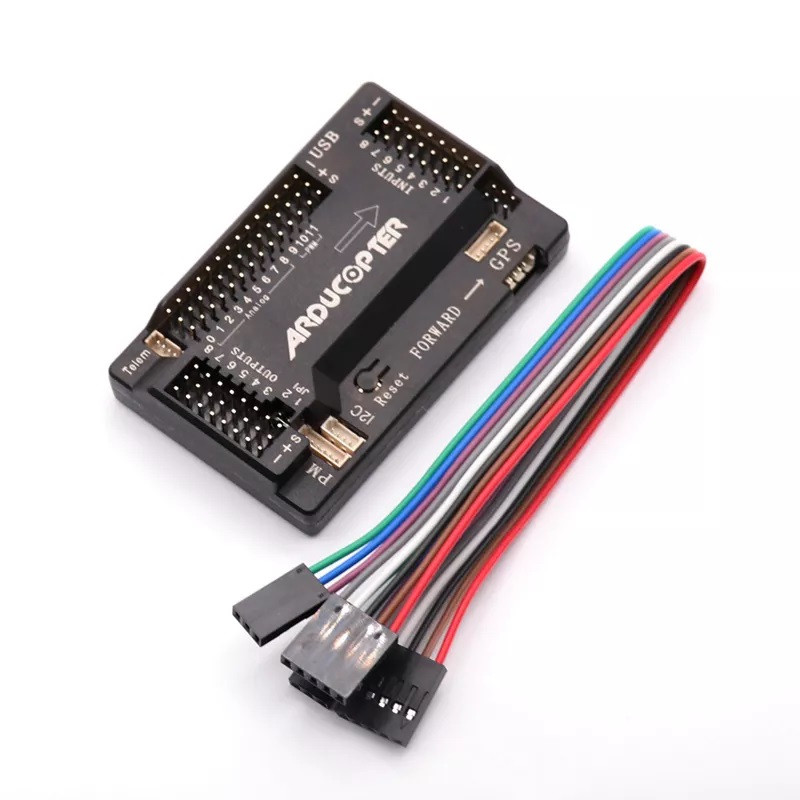
\includegraphics[width=0.3\linewidth]{Images/controlleur-de-vol-ardupilot-apm28}}
	\end{center}
	\caption{APM 2.8}
\end{figure}

\subsection {Radiocomamande}
Une radiocommande est un outil permettant de contrôler à distance notre drone à travers des signaux radio. Nous avons choisi cet appareil grâce à sa portée et sa latence qui sont importantes par rapport au wifi et au bluetooth. Son émetteur est de type Turnigy 9x et son récepteur de type IA8 AFHDS2A.

\subsubsection{Émetteur} 
La Turnigy 9x est une radiocommande de 9 voies, elle est équipée de 6 interrupteurs de deux positions, un interrupteur de trois position et de trois potentiomètres rotatifs.
De plus, grâce à la technologie 2,4 Ghz, nous disposons d'une réaction ultra-rapide et d'un contrôle sans interférence. Pour la
conception ergonomique, celle-ci facilite l'utilisation de toutes les commandes dont les interrupteurs et les ports sont tous positionnés pour plus de confort \cite{Hobbyking}. En plus, les bâtons de longueur réglable peuvent être adaptés à nos besoins et l' écran LCD monochrome facilite la programmation ainsi que la modification des paramètres. 

\begin{figure} [H]
	\begin{center}
		\centering
		\fbox{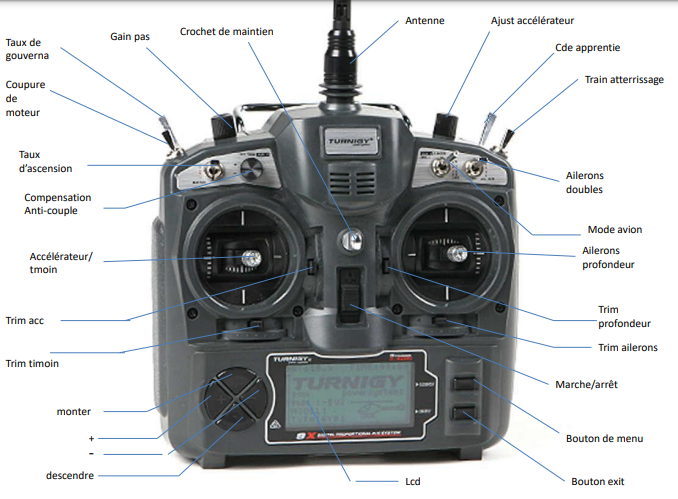
\includegraphics[width=0.8\textwidth]{Images/Emetteur radiocommande}}
	\end{center}
	\caption{Turnigy 9x}
\end{figure}
\subsubsection{Récepteur }
Ce récepteur IA8 AFHDS 2A dispose de 8 voies et fonctionne parfaitement avec la radiocommande Turnigy 9x système AFHDS 2A \cite{Hobbyking}. Il a une portée de plus de 500 mètres  grâce à ses deux antennes. En plus, ce composant reste très compact et fonctionne en PWM ou PPM.
\begin{figure} [H]
	\begin{center}
		\centering
		\fbox{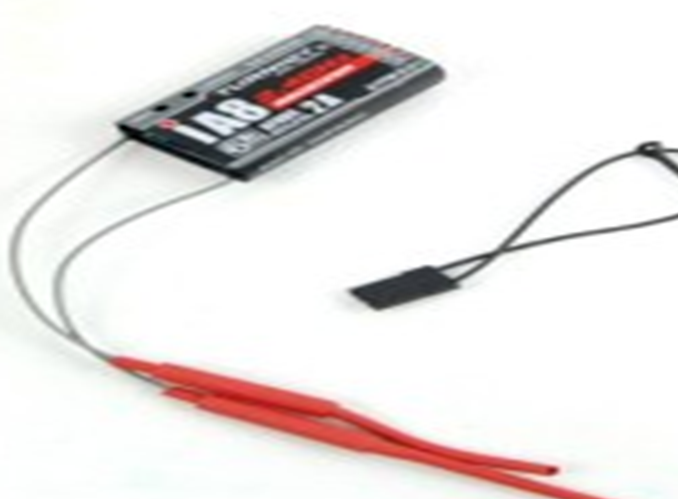
\includegraphics[width=0.4\textwidth]{Images/Récépteur radiocommande}}
	\end{center}
	\caption{Récepteur IA8 AFHDS 2A}
\end{figure}
\subsection {Diodes  et résistances}
Afin d'éclairer notre quadrirotor, nous avons utilisé 8 diodes ( 4 diodes blanches et 4  rouges) pour mieux connaître son mouvement. Nous avons utilisé 5V de l'APM 2.8. Puisqu'une diode a besoin de 3V et 5mA, nous avons choisi une résistance de \SI{330}{\ohm} à chaque diode pour encaisser les 2V supplémentaires et tout cela sous 5mA.
\begin{figure}[H]
	\centering
	\begin{minipage}{0.49\textwidth}
		\hspace*{-0.7cm}
		\fbox{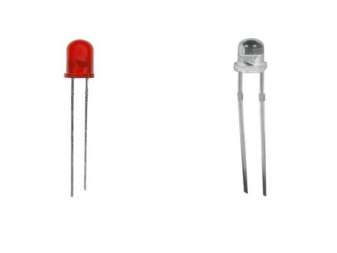
\includegraphics[width=0.8\textwidth]{Images/Diodes (blanche et rouge)}}
		\centering
		\caption{Diodes}
		\label{fig:my_label}
	\end{minipage}
	\begin{minipage}{0.49\textwidth}
		\hspace*{0.2cm}	\fbox{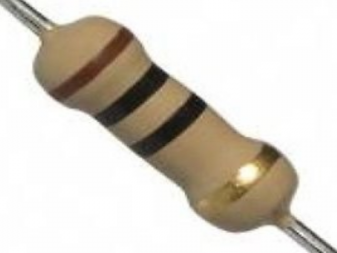
\includegraphics[width=0.8\textwidth]{Images/Résistance 330Ω}}
		\centering
		\caption{Résistance}
		\label{fig:my_label}
	\end{minipage}
\end{figure}

\section{Diagramme de bloc de définition  }

Le diagramme de définition de bloc permet d'exprimer la structure d'un système, d'un sous-système ou d'un composant. Ces blocs peuvent représenter des entités physiques ou logiques qui sont décomposables et peuvent posséder des propriétés ainsi qu'un comportement \cite{siloged}.


\begin{figure}[H] 
	\begin{center} 
		\centering
		\hspace*{-0.4cm}	\fbox{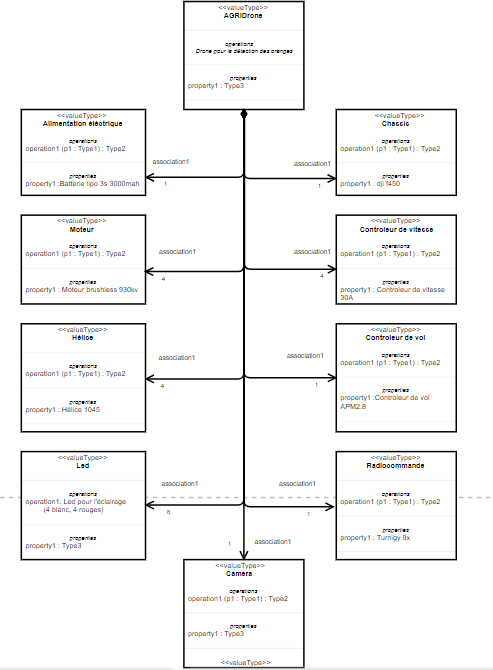
\includegraphics[width=1.15\linewidth]{Images/Diagramme de définition de bloc}}
	\end{center}
	
	\caption{Diagramme de définition de bloc}
	
	\end {figure}
	Notre AGRIDrone  est constitué de plusieurs éléments. Il existe deux principaux blocs: le quadrirotor et le système de détection.
	
	Le quadrirotor est lié à une alimentation électrique qui  délivre une tension de 12V au contrôleur de vitesse. Ce dernier transmet 5V au contrôleur de vol qui l'envoi à son tour au récepteur de la radiocommande afin de l'allumer. Ce composant est en attente du signal radio qui va être transmis par l'émmeteur. Dès que ce signal est reçu, le récepteur se charge de le décoder puis de l'envoyer au contôleur de vol en tant que signal PWM. Par la suite, il sera transmis au contrôleur de vitesse pour effectuer le démarrage des moteurs qui sont chargés de la rotation des hélices. Le châssis est aussi un élément du quadrirotor qui supporte tous ses composants sauf l'émetteur de la radiocommande.
	
	Concernant le système de détection, il est aussi en relation avec l'alimentation électrique. Cette dernière fournit une tension de 12V au système de décision qui délivre 5V à la caméra.
	\section{Logiciels utilisés}
	Dans notre projet, nous avons travaillé sur de nombreux logiciels que nous traitons un par un.
	\subsection{Latex}
	Nous avons choisi comme éditeur de texte le logiciel "Latex" car il nous  offre de nombreuses fonctionnalités et nous permet de composer une très grande variété de formules mathématiques.
	\begin{figure}[H]
		\begin{center}
			\centering
			\fbox{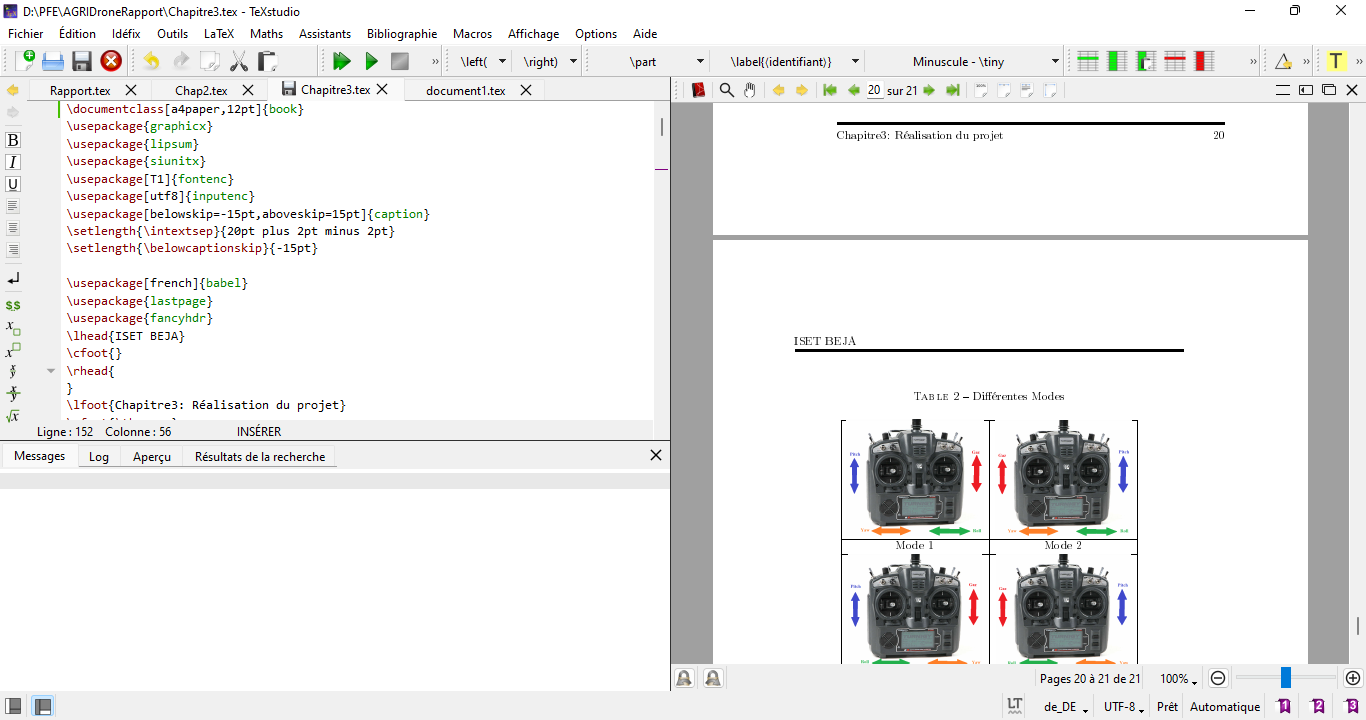
\includegraphics[width=0.6\linewidth]{Images/Latex}}
		\end{center}
		\caption{Interface de Latex}
	\end{figure}
	\subsection{Google Drive}
	Dans le but de partager en collaborant notre travail, nous avons utlilisé "google drive" qui nous permet de travailler sur les différents documents à produire au cours du projet.
	\begin{figure}[H]
		\begin{center}
			\centering
			\fbox{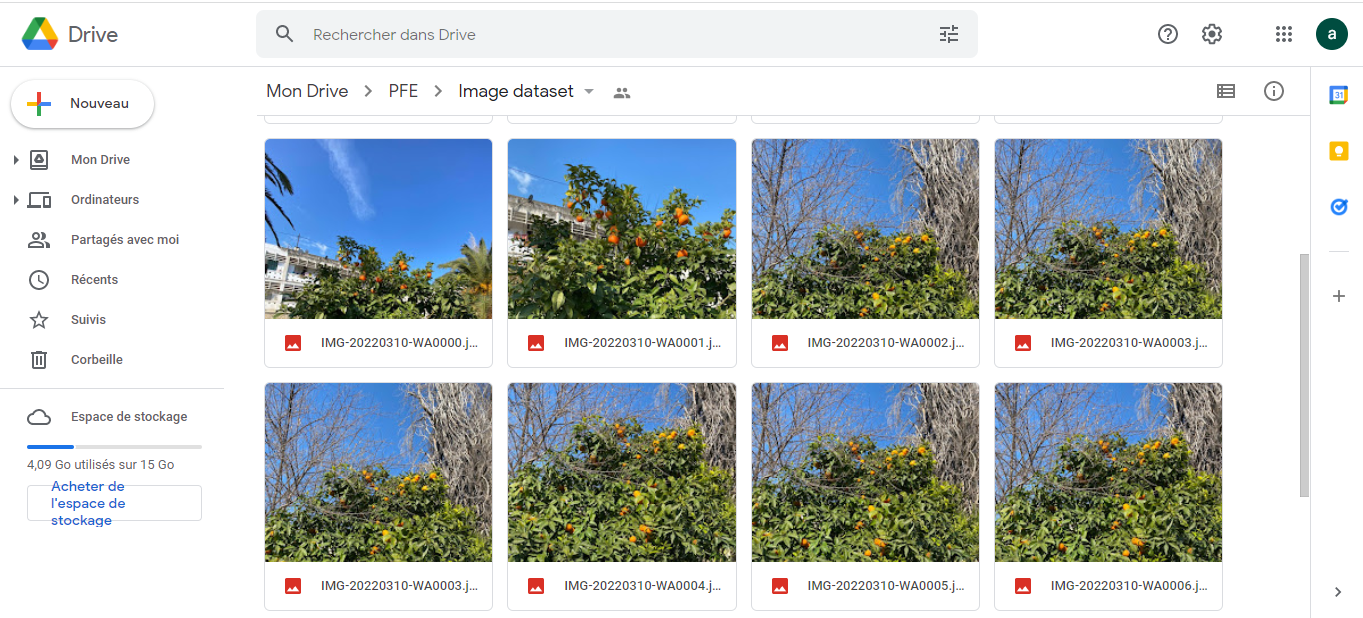
\includegraphics[width=0.6\linewidth]{Images/Google drive}}
		\end{center}
		\caption{Plateforme sur Google drive}
	\end{figure}
	\subsection{Jira Software}
	Nous avons sélectionné "jira software" comme étant un outil de gestion de notre projet puisqu'il est  puissant et nous permet de visualiser l'avancement de notre travail grâce aux tableaux Agile. En plus, il nous offre la possibilité de travailler à distance grâce à cette plateforme.
	\begin{figure}[h]
		\begin{center}
			\centering
			\fbox{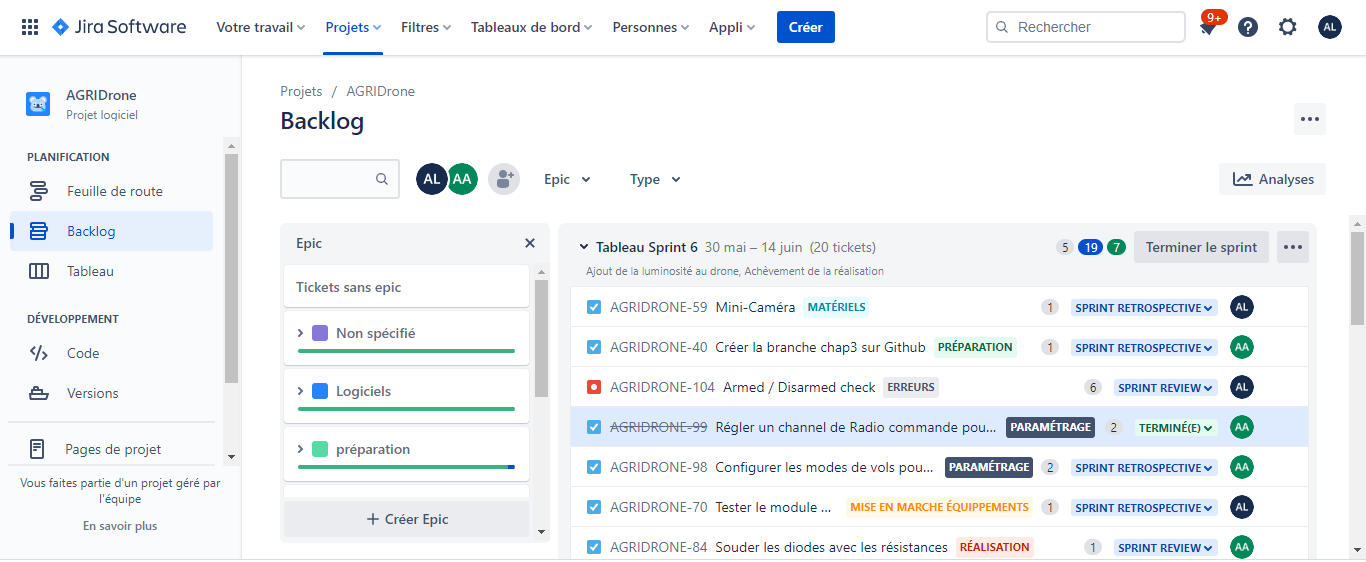
\includegraphics[width=0.6\linewidth]{Images/Jira}}
		\end{center}
		\caption{Plateforme sur Jira software}
	\end{figure}
	\subsection{GitHub}
	C'est un service web que nous avons utilisé pour la centralisation et la gestion de notre rapport puisqu'il nous garantit la sauvegarde des versions  que nous avons traité précédemment et le gain en temps à travers la répartition des tâches.  
	
	\begin{figure}[H]
		\begin{center}
			\centering
			\fbox{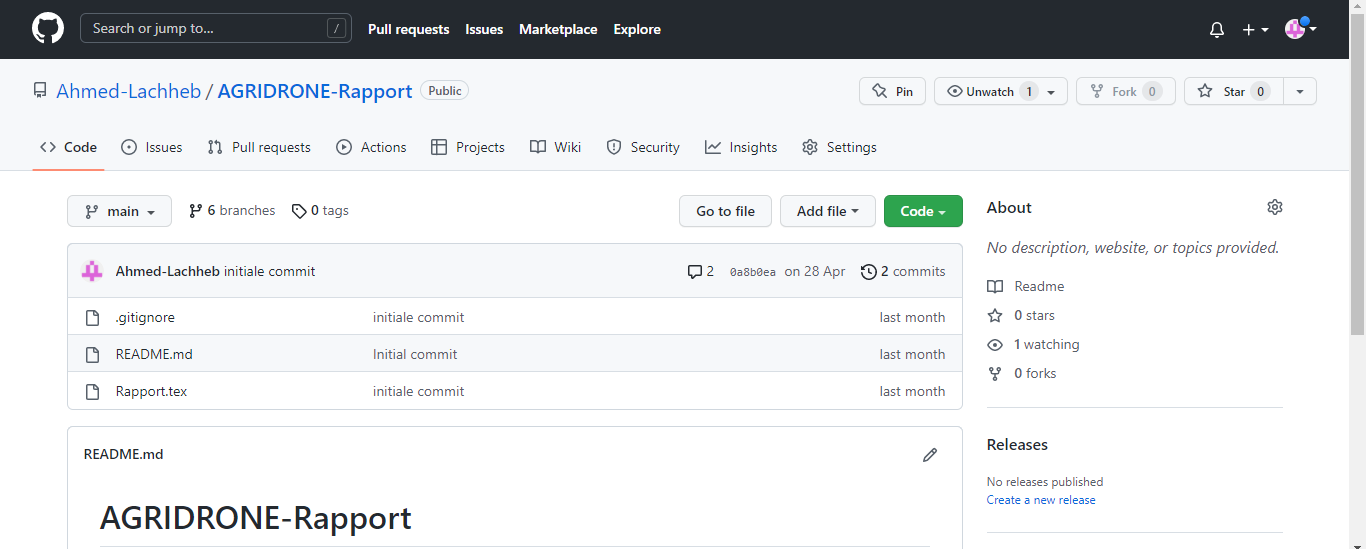
\includegraphics[width=0.7\linewidth]{Images/Github}}
		\end{center}
		\caption{Plateforme sur GitHub}
	\end{figure}
	\subsection{Papyrus}
	C'est un logiciel gratuit qui est riche en fonctionnalités. Il nous a aidé à faire la conception de notre projet à travers les diagrammes de cas d'utilisation.
	\begin{figure}[H]
		\begin{center}
			\centering
			\fbox{\includegraphics[width=0.7\linewidth]{Images/Papyrus}}
		\end{center}
		\caption{Interface Papyrus}
	\end{figure}
	
	\subsection{Visual Paradigm}
	Suite à des obstacles que nous avons rencontré au niveau de Papyrus, nous avons recours à "Visual Paradigm" pour la réalisation des diagrammes d'exigence et de définition de bloc.
	\begin{figure}[H]
		\begin{center}
			\centering
			\fbox{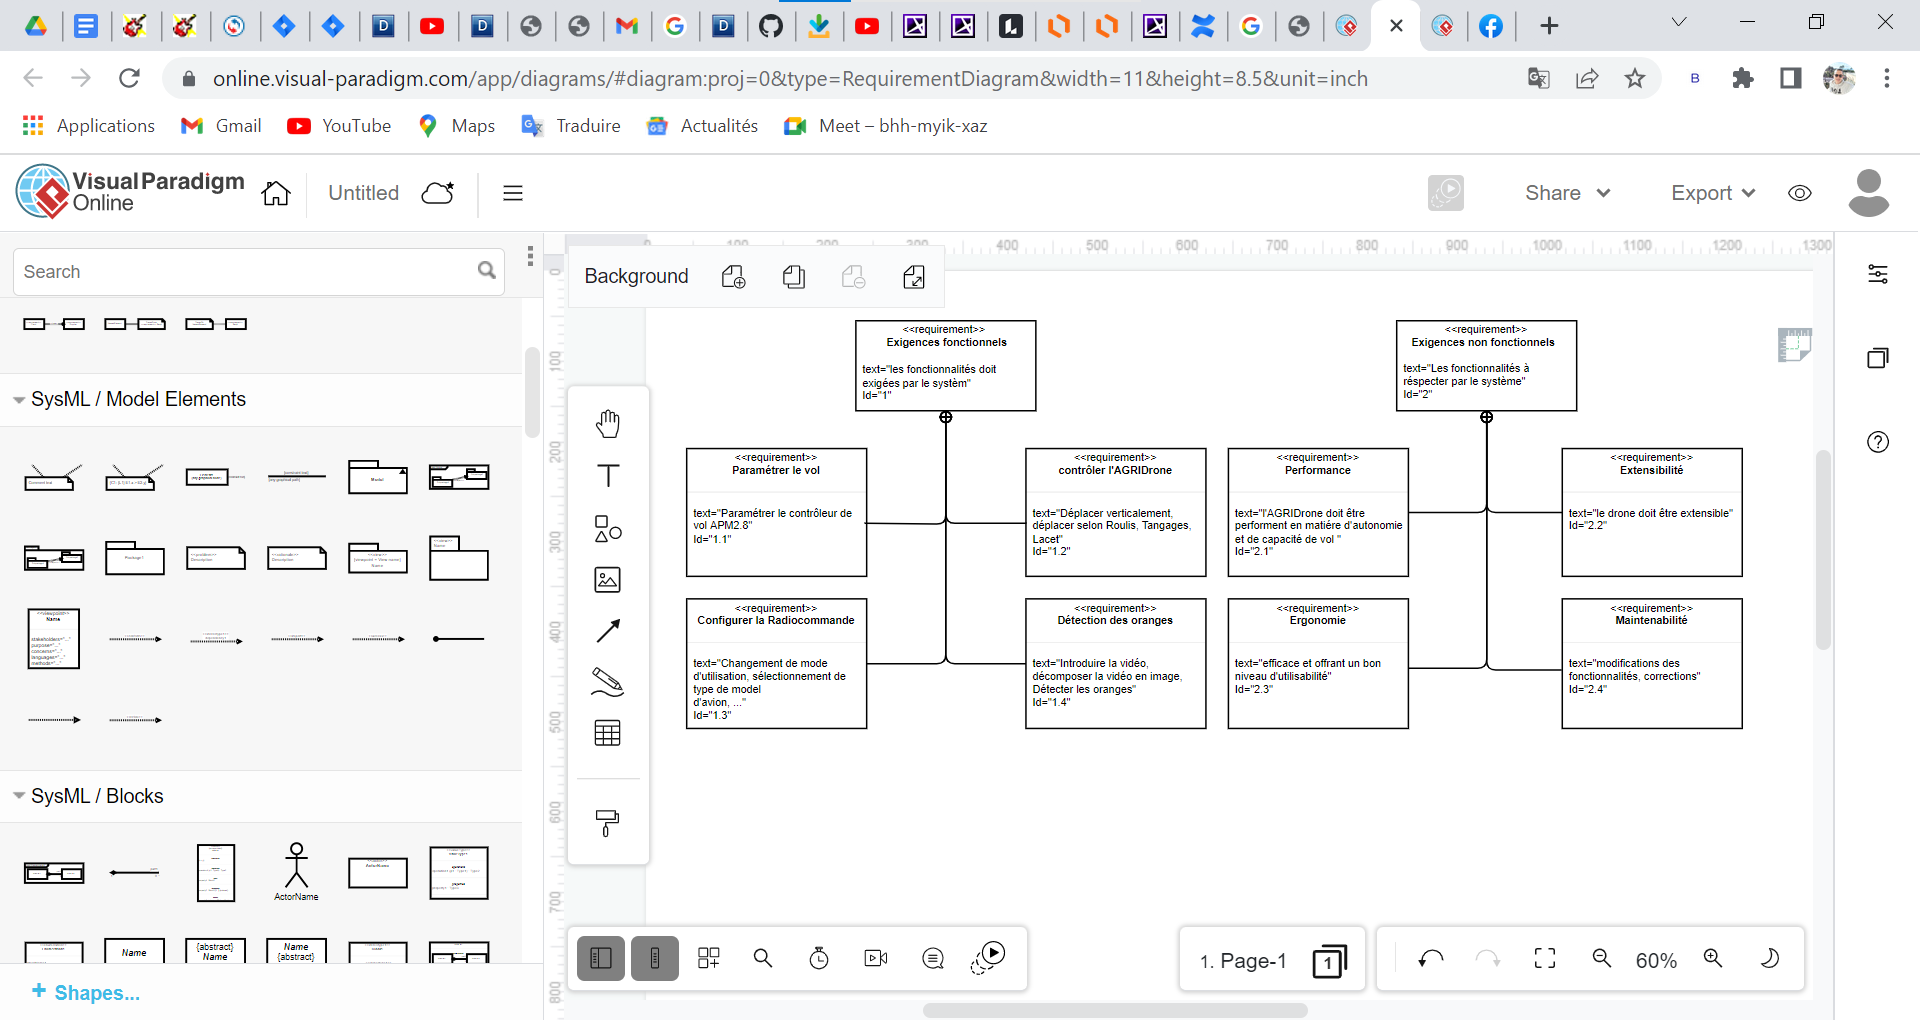
\includegraphics[width=0.7\linewidth]{Images/Visual Paradigm}}
		\end{center}
		\caption{Interface Visual Paradigm}
	\end{figure}
	\subsection{Companion 9x}
	Nous avons utilisé ce logiciel pour téléverser le firmware vers la mémoire de l'émetteur du radiocommande.
	\begin{figure}[H]
		\begin{center}
			\centering
			\fbox{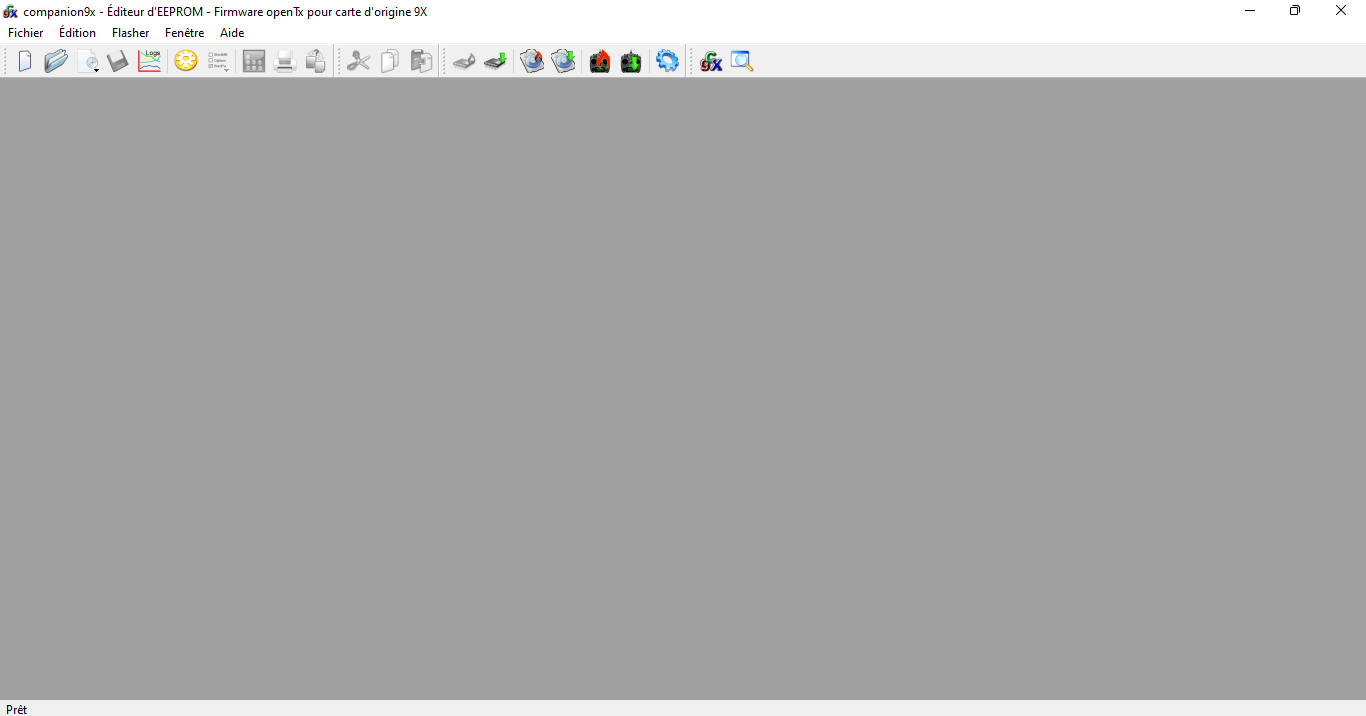
\includegraphics[width=0.7\linewidth]{Images/Companion 9x}}
		\end{center}
		\caption{Interface de Companion 9x}
	\end{figure}
	
	\subsection{JabRef}
	"JabRef" est un logiciel que nous avons utilisé dans la gestion bibliographique. Il nous fournit une interface conviviale pour éditer des fichiers Bib(La)TeX.
	\begin{figure}[H]
		\begin{center}
			\centering
			\fbox{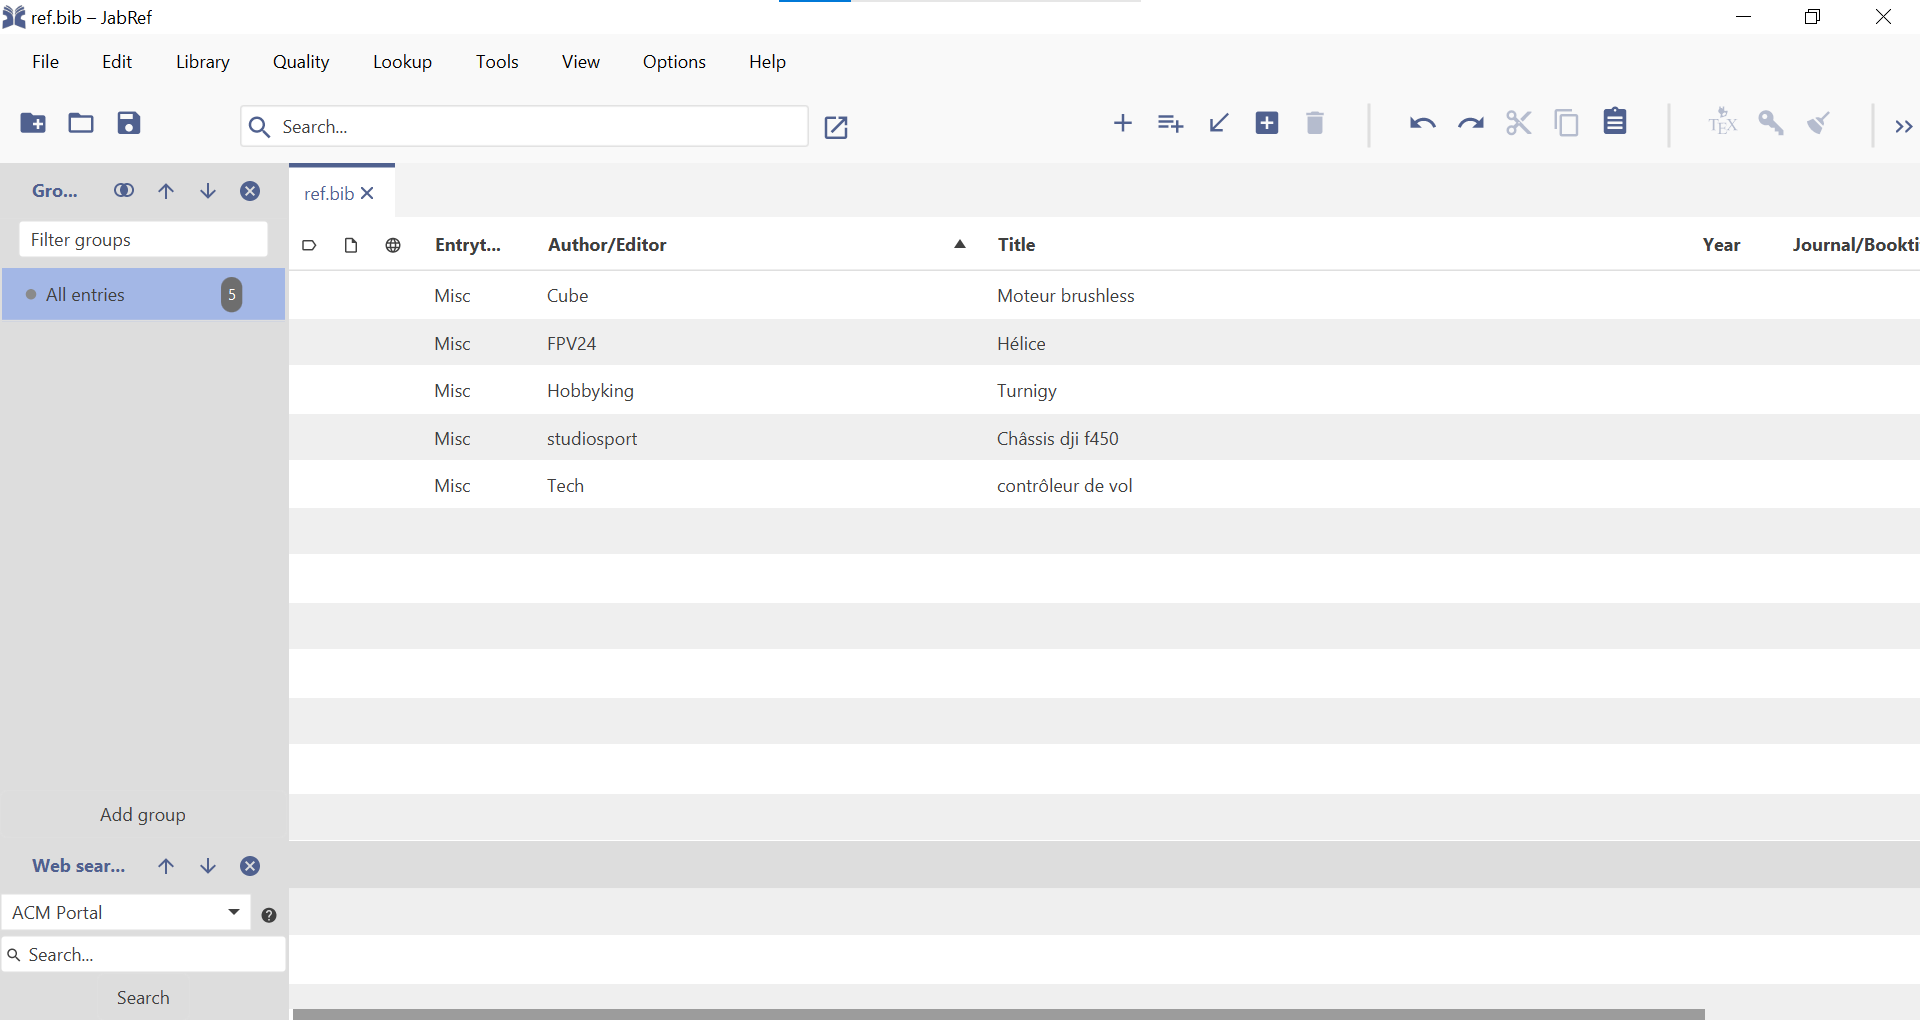
\includegraphics[width=0.6\linewidth]{Images/Platforme de JabRef}}
		\end{center}
		\caption{Interface du Jabref}
	\end{figure}
	\subsection{Mission Planner	}
	Ce logiciel représente une station de contrôle au sol pour les hélicoptères, avions ou rovers. Il nous a permis de paramétrer notre contrôleur de vol et de configurer ses différents paramètres ainsi que d'assurer ses performances optimales.
	\begin{figure} [H]
		\begin{center}
			\centering
			\hspace*{1.5cm}\fbox{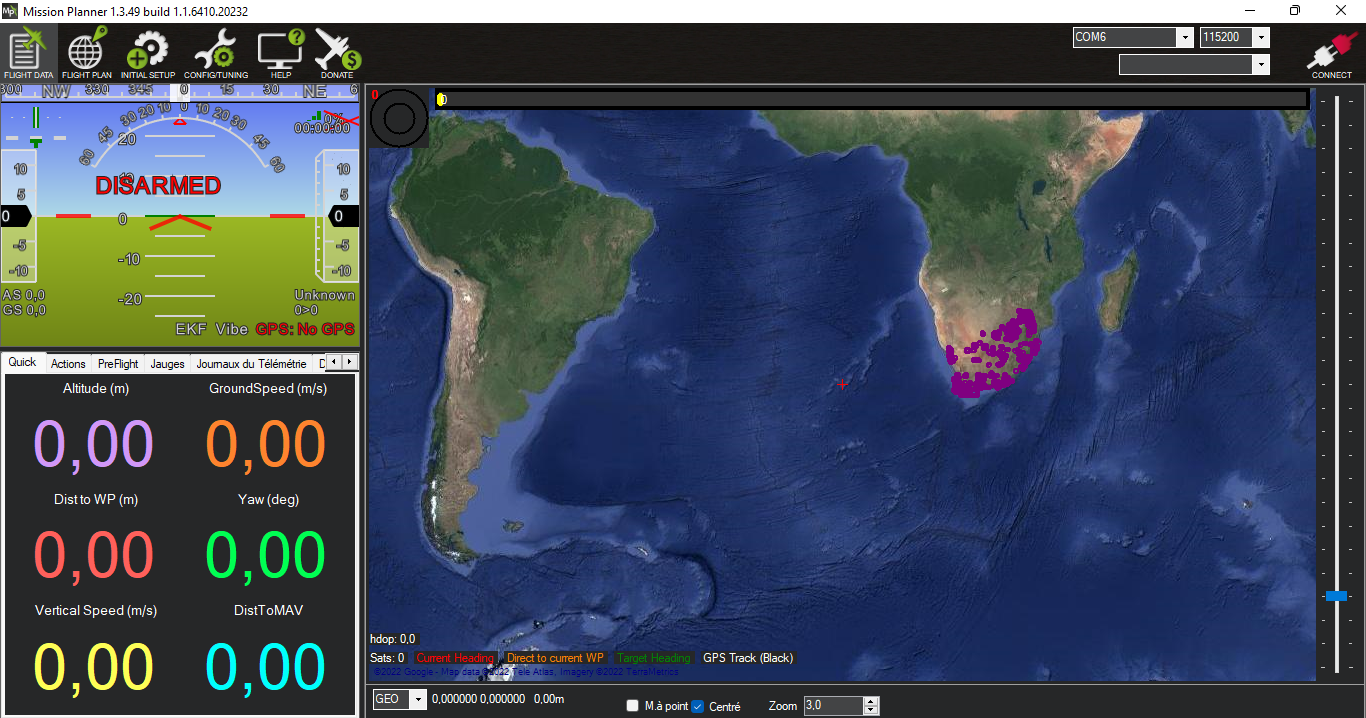
\includegraphics[width=0.65\linewidth]{Images/Interface de Mission Planner}}
			\centering
			\hspace*{1.5cm}	\caption{Interface de Mission Planner}
		\end{center}
	\end{figure}
	
	\section{Montage des composants}
	Pour réaliser notre drone, on a poursuivi le schéma électrique présenté ci-dessous :
	
	\begin{figure} [H]
		\begin{center}
			\centering
			\hspace*{-1cm}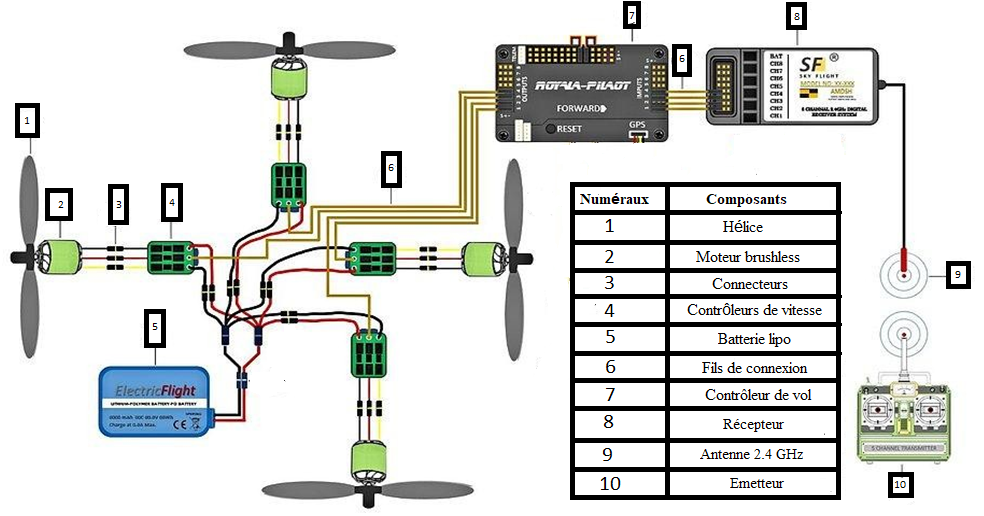
\includegraphics[width=1.1\linewidth]{Images/Shéma électrique}
		\end{center}
		\caption{Montage des composant}
	\end{figure}
	
	
	\section{Configurations et calibrations}
	Puisque le contrôleur de vol et la radiocommande fonctionnent sur différents modèles d'avions, il est nécessaire de leurs effectuer des configurations  ainsi que  des calibrations spécifiques pour le fonctionnement de notre quadrirotor. 
	\subsection{Configurations et calibrations de l'APM 2.8}
	Pour configurer et calibrer l'"APM 2.8", nous devons lancer l'assistant et le connecter en USB sur notre PC.
	\subsubsection{Chargement du firmware }
	Ensuite, nous avons accédé au « INITIAL SETUP ». L'installation du firmware se fait en cliquant sur le bouton « Install Firmware ». Cette opération commence après avoir sélectionné le type du multicoptère, dans notre cas c'est le « quadrirotor » que nous avons chargé. La dernière version du firmware dans
	notre carte "APM2.8" est présentée dans la figure ci-dessous. Le logo « CONNECT » doit rester rouge c'est à dire en mode déconnecté. Dès que le firmware est installé, le drone sera prêt à être configuré et paramétré.
	\begin{figure}[H]
		\begin{center}
			\centering
			\fbox{ 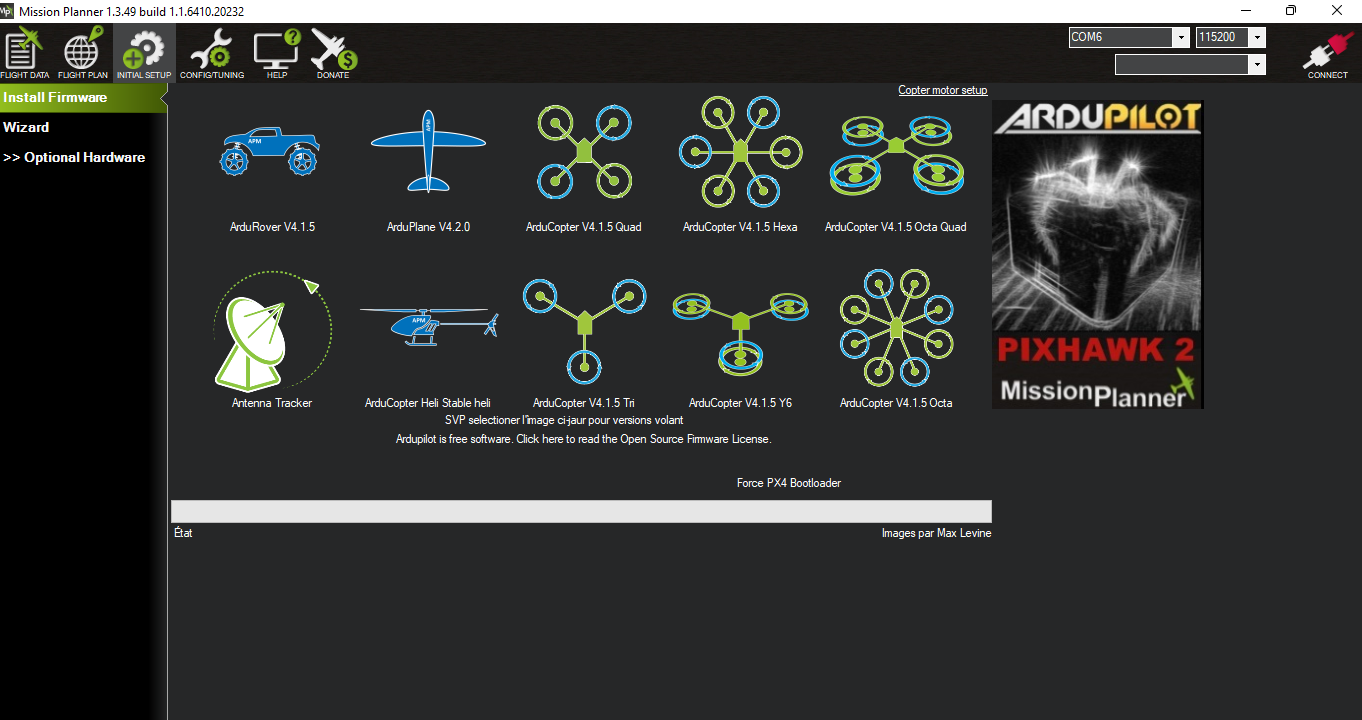
\includegraphics[width=0.6\linewidth]{Images/Chargement du firmware}}
		\end{center}
		\caption{Chargement de firmware}
	\end{figure}
	
	\subsubsection{Type de châssis}
	Après avoir installé le firmware, nous avons connecté  la carte "APM 2.8" en haut à droite de Mission Planner. Pour s'assurer que notre carte est bien connectée, le logo « CONNECT » doit passer de la couleur rouge à la couleur verte. Ensuite, nous avons cliqué sur « INITIAL SETUP », « Mandatory Hardware » et « Frame Type » afin de configurer le type de notre quadrirotor. 
	\begin{figure}[H]
		\begin{center}
			\centering
			\fbox{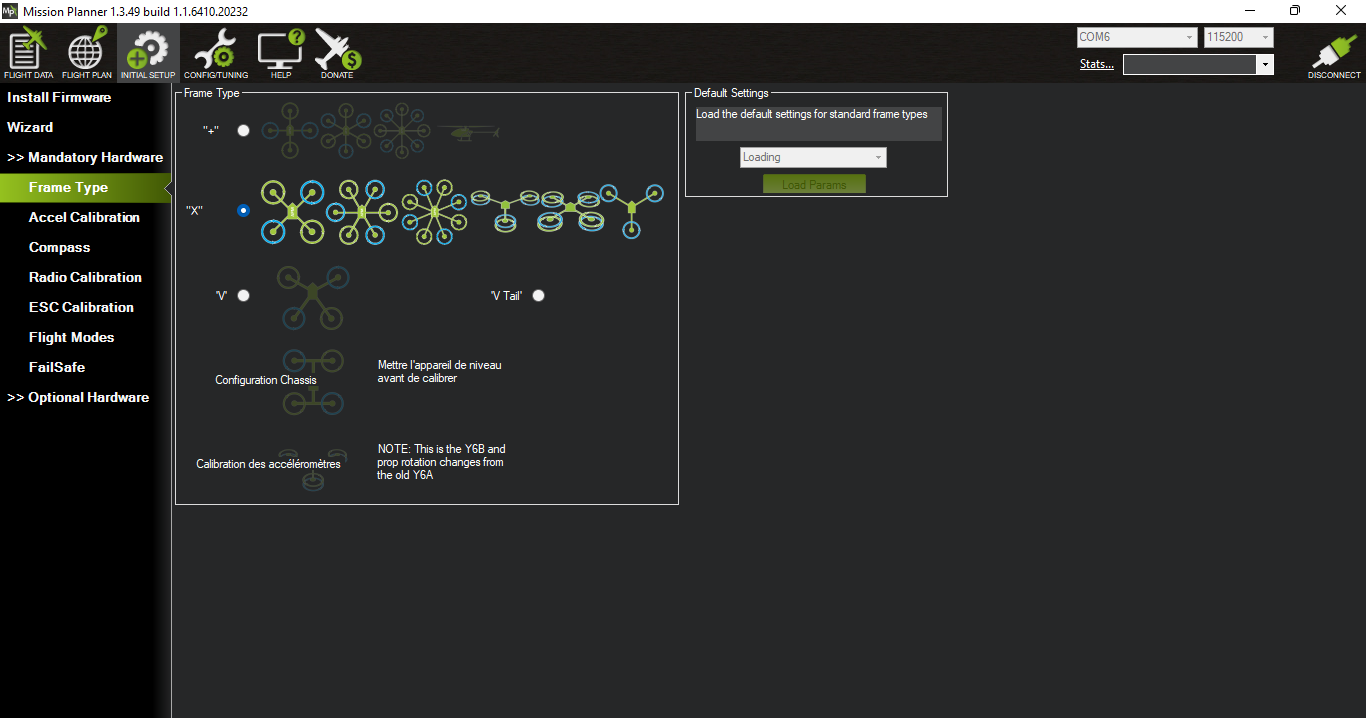
\includegraphics[width=0.53\linewidth]{Images/Choix du type de quadrirotor}}
		\end{center}
		\caption{Choix du type de châssis}
	\end{figure}
	\subsubsection{Calibration du magnétomètre}
	Pour réaliser cette manipulation, il est préférable de connecter le contrôleur de vol avec un câble USB afin d'obtenir un échantillonnage précis et continu.
	Dans la sous-section « Compass », il vaut mieux vérifier que le magnétomètre est activé ainsi que la déclinaison soit automatique.
	
	\begin{figure}[H]
		\begin{center}
			\centering
			\fbox{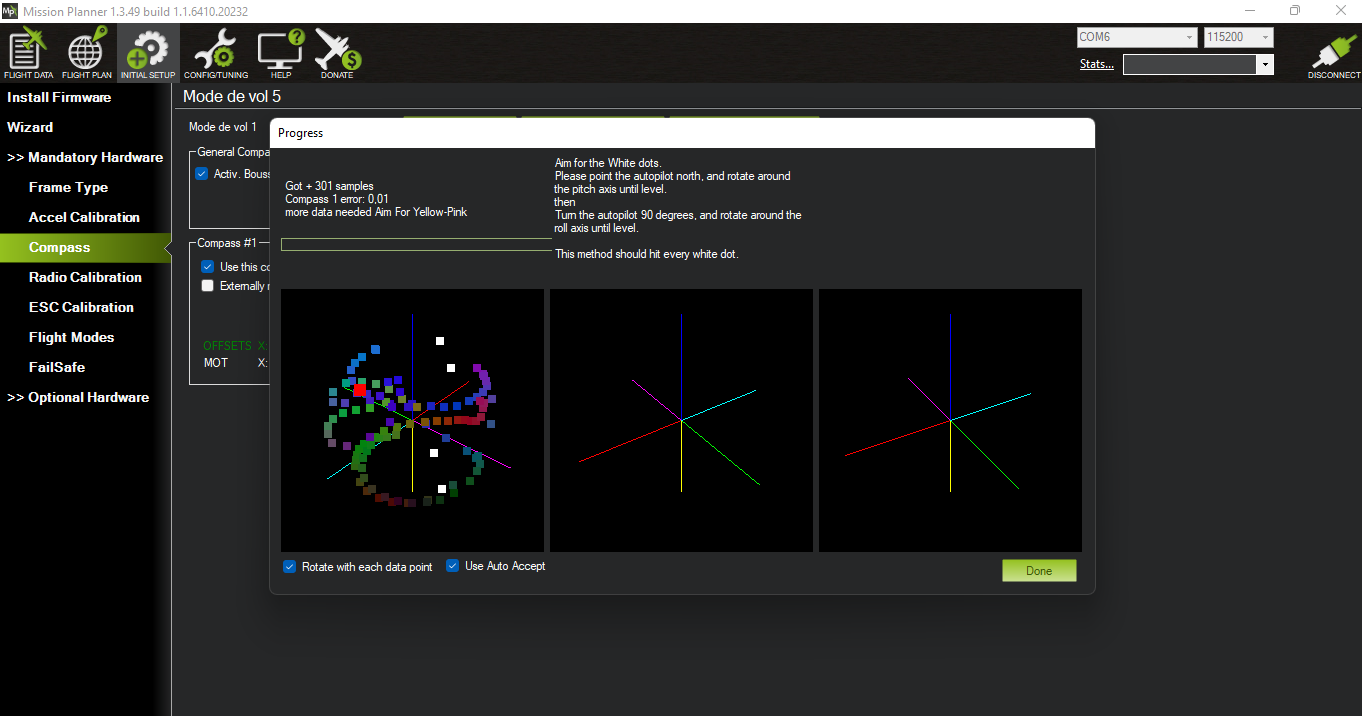
\includegraphics[width=0.53\linewidth]{Images/calibration du magnétométre}}
		\end{center}
		\caption{Calibration du magnétométre}
	\end{figure}
	
	\subsubsection{Calibration des accéléromètres}
	Pour un résultat optimal,  nous devons premiérement  accéder au menu « INITIAL SETUP », deuxièment « Mandatory Hardware » et finalement, « Accel Calibration ». L'"APM2.8" doit être positionnée successivement sur chacune de ses six faces.
	La séquence se présente de la façon suivante :
	
	\begin{table}[H]
		\begin{center}
			
			\vspace{1cm}\caption{Calibration des accéléromètres  }
			
			\hspace*{-1.1 cm}	\begin{tabular}{|c|c|}
				\hline
				\centering
				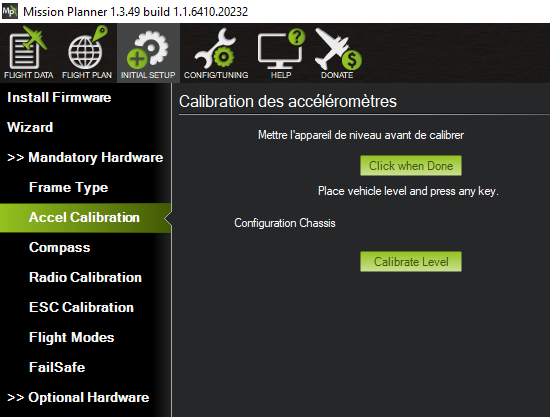
\includegraphics[width=7.5cm]{Images/A plat sur le ventre} & 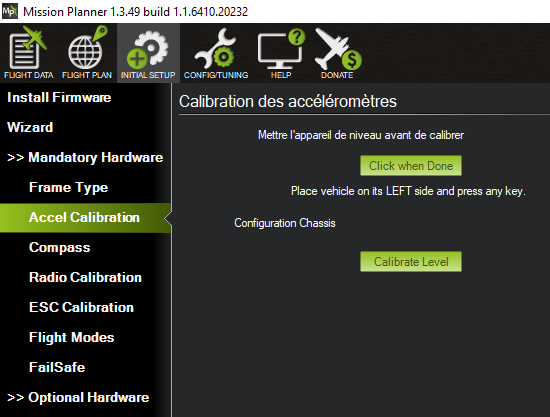
\includegraphics[width=7.5cm]{Images/Vertical sur son flanc gauche}\\
				\hline
				\centering
				
				1) A plat sur le ventre & 2) Vertical sur son flanc gauche \\
				
				\hline
				
				
				\centering
				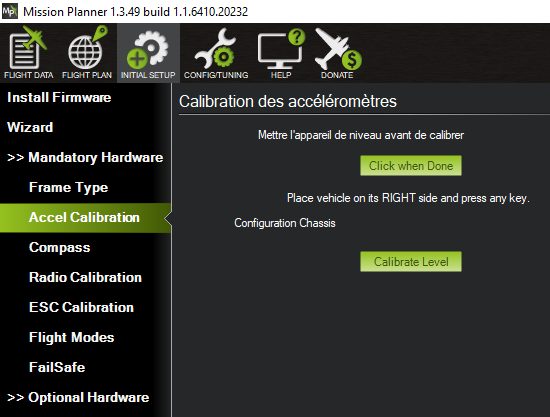
\includegraphics[width=7.5cm]{Images/Vertical sur son flanc droit} & \includegraphics[width=7.5cm]{Images/Nez en bas}
				\\
				\hline
				
				
				\centering
				3) Vertical sur son flanc droit &   4) Nez en bas \\
				\hline
				
				
				\centering
				\includegraphics[width=7.5cm]{Images/Nez en l’air} & \includegraphics[width=7.5cm]{Images/Sur le dos}\\
				\hline
				\centering
				
				5) Nez en l’air &   6) Sur le dos \\
				\hline
			\end{tabular}
		\end{center}
	\end{table}	
	
	
	
	\subsubsection{Calibration du radiocommande}
	Après s'être assuré que le récepteur est bien connecté au contrôleur de vol et qu'il est apparié à la radiocommande sous tension et correctement programmée, nous avons  accédé aux « Radio Calibration », cliqué sur le bouton « Calibrer Radio ». 
	Une fois validé, nous avons actionné toutes les commandes de la radio de leur minimum à leur maximum. 
	\begin{figure} [H]
		\begin{center}
			\centering
			\fbox{\includegraphics[width=0.8\linewidth]{Images/calibaration du radio}}
		\end{center}
		\caption{Calibration du radiocommande}
	\end{figure}
	
	\subsubsection{Configurations des modes de vol} 
	Notre "APM 2.8" est caractérisé par la variété de ces modes de vol qui nous facilitent le pilotage et le contrôle de notre quadrirotor. Dans notre cas, nous avons utilisé deux modes de vol: le mode « Stabilize » nous permettant de contrôler notre drone manuellement et le mode « Alt Hold » permet le maintien de l'altitude constante. A savoir, le mode « Alt Hold » n'est pas applicable vu l'absence de GPS. Pour effectuer  cette configuration, nous avons accédé au « Flight Modes » comme le montre la figure ci-dessous.
	
	\begin{figure} [H]
		\begin{center}
			\centering
			\fbox{\includegraphics[width=0.8\linewidth]{Images/Modes de vol}}
		\end{center}
		\caption{Modes de vol}
	\end{figure}
	
	\subsubsection{Régulateurs PID de contrôleur de vol APM2.8}
	Dans le contrôleur de vol que nous avons utilisé, à savoir Ardupilot "APM 2.8" des régulateurs PID sont implantés automatiquement lors de la téléchargement du firmware de quadrirotor.
	
	Voici la fenêtre de configuration des PIDs de l'Ardupilot suivante :
	\begin{figure} [H]
		\begin{center}
			\centering
			\fbox{\includegraphics[width=0.8\linewidth]{Images/PID APM 2.8}}
		\end{center}
		\caption{Les valeurs des PIDs de l'APM 2.8}
	\end{figure}
	
	\subsubsection{Calibration des ESC}
	Les contrôleurs de vitesse doivent être étalonnés pour connaître les valeurs minimales et maximales du commande des gaz. 
	
	Concernant La procédure d’étalonnage, nous avons en premier lieu coupé l'alimentation de l'appareil. Par la suite, nous avons allumé la radiocommande et positionné le manche des gaz à son maximum. Ensuite, nous avons mis l'appareil sous tension en attendant que le contrôleur de vol démarre. Ainsi, nous avons coupé l'alimentation de l'appareil et nous l'avons remis sous tension. Après avoir entendu la mélodie issue des moteurs confirmant l'apprentissage de la valeur maximale des gaz, nous avons baissé le manche des gaz au minimum en attendant la mélodie de confirmation et actionner doucement les gaz pour vérifier que tous les moteurs démarrent en même temps et tournent au même régime. Finalement, nous avons recoupé l'alimentation de l'appareil.
	\subsection{Configuration et calibration de la radiocommande}
	Concernant la configuration et la calibration de la radiocommande, nous avons passé par plusieurs étapes que nous expliquons ci-dessous. 
	\subsubsection{Mode de la radiocommande}
	Au début, notre radiocommande est activée en mode "1" où le bâton droite est relâché dans l'axe verticale et le bâton gauche est centré dans les deux axes. Afin de faciliter le pilotage de notre drone, nous avons activé notre radiocommande en mode "2" qui est l'inverse du mode précédent. Pour effectuer cette opération, nous avons tout d'abord retiré les six vis à l'arriére du boîtier. Ensuite, nous avons déplacé le ressort vers le bâton droite. Finalement, nous avons fermé la radiocommande en remettant les vis.
	
	
	\subsubsection{Type de modèle}
	Cette fonctionnalité nous permet de sélectionner le type de modèles réduits d'avions qui seront utilisés ou affectés à un modèle particulier.
	Dans le menu Réglages Système, nous avons sélectionné « SELE TYPE » et appuyé sur « MENU ». Ensuite, en utilisant le haut ou bas nous avons choisi le type de modèle qui sera utilisé soit HELI, ACRO ou bien GLID. Après avoir sélectionné l'option Acro, nous avons appuyé sur « MENU  » pour enregistrer, puis sur « EXIT » pour retourner au menu précédent.
	
	\begin{figure}[H]
		\begin{center}
			\centering
			\fbox{\includegraphics[width=0.6\linewidth]{Images/Type de modèle}}
		\end{center}
		\caption{Type de modèle}
	\end{figure}
	\subsubsection{ Type de modulation}
	Cette fonctionnalité nous permet de sélectionner le type de modulation qui sera utilisé à un modèle particulier (PPM ou PCM).
	
	
	\textbf{PPM:} modulation de position d'impulsion. 
	
	\textbf{PCM:} modulation d'impulsions codées.
	
	
	Dans le menu configuration système, nous avons cliqué sur « Modeuat », appuyé sur « MENU », sélectionné l'option désirée PPM et confirmé cette option sélectionnée en appuyant sur « MENU ». Ensuite, nous avons appuyé sur le bouton « EXIT » pour revenir au menu précédent.
	
	\begin{figure}[H]
		\begin{center}
			\centering
			\fbox{\includegraphics[width=0.6\linewidth]{Images/Sélection de mode pour Acro}}
		\end{center}
		\caption{Sélection de mode pour Acro}
	\end{figure}
	\subsubsection{Mode de la radiocommande }
	Dans le menu Réglages Système, nous avons sélectionné « STICK SET », après avoir presser le « MENU ». Ensuite, nous avons choisi le mode le plus appropriée à notre style d'utilisation "modèle 2". Dés que cette étape est réalisée, nous avons effectué la sauvegarde de l'option sélectionnée en appuyant sur « MENU ». Après, nous avons appuyé sur le bouton «EXIT» pour revenir au menu précédent.
	\begin{figure}[H]
		\begin{center}
			\centering
			\fbox{\includegraphics[width=0.6\linewidth]{Images/Les 4 modes}}
		\end{center}
		\caption{Les 4 modes}
	\end{figure}
	
	Après avoir visualisé les différents modes de pilotage, nous allons les traiter un par un à travers le tableau suivant:
	
	\begin{table}[H]
		\begin{center}
			
			\vspace{1cm}	\caption{Différentes Modes }
			\begin{tabular}{|c|c|}
				\hline
				
				\centering
				
				\includegraphics[width=4.74cm]{Images/Mode 1(Radiocommande)} & \includegraphics[width=4.8cm]{Images/Mode 2(Radiocommande)}\\
				\hline
				\centering
				
				Mode 1 & Mode 2 \\
				
				\hline
				\centering
				\includegraphics[width=4.69999cm]{Images/Mode 3(Radiocommande)}& \includegraphics[width=4.69999cm]{Images/Mode 4(Radiocommande)}\\
				\hline
				\centering
				
				Mode 3 &  Mode 4 \\
				\hline
			\end{tabular}
		\end{center}
	\end{table}
	
	
	
	
	\subsubsection{Inversion des servos}
	La Servo Reverse nous permet de renverser le fonctionnement du servos afin de le manipuler conformément à nos besoin.
	
	
	
	Dans le MENU REGLAGES nous avons appuyé sur « FUNC » et sélectionné la fonction « REVERSE » en utilisant les touches haut ou bas. Ensuite, avec les touches + ou -
	nous avons appliqué cette fonction aux servos que nous avons affécté à cette opération. Aprés, nous avons appuyé sur « MENU » pour sauvegarder les nouveaux réglages et revenir au menu précédent.
	\begin{figure}[H]
		\begin{center}
			\centering
			\fbox{\includegraphics[width=0.6\linewidth]{Images/Inversion des servos}}
		\end{center}
		\caption{Inversion des servos}
	\end{figure}
	\section{Erreur eeprom}
	Lors de la configuration et du paramétrage de notre radiocommande, nous avons observé qu'elle s'éteind tout d'un coup et un message "erreur eeprom" s'affiche avec une alerte sonore. Nous avons effectué le redémarrage de la radiocommande mais en vain. Nous avons cherché comment résoudre ce problème et nous avons constaté qu'il faut la rènitialiser. Pour effectuer cette opération, nous avons besoin d'un logiciel, d'un firmware à installer et d'un programmateur.
	\subsection{Microcontôleur Green-128}
	L'emmetteur de notre radiocommande turnigy 9x contient un microcontrôleur "Green-128" qui est compatible avec le microcontrôleur  "Atmega 128". Nous montrons dans la figure ci-dessous les pins de "Green-128". 
	\begin{figure}[H]
		\begin{center}
			\centering
			\fbox{\includegraphics[width=0.5\linewidth]{Images/Green-128}}
		\end{center}
		\caption{Pins Green-128\label{fig:P.G}}
	\end{figure}
	
	\subsection{Programmateur Usbasp}
	Puisque le microcontrôleur "Green-128" est compatible avec "Atmega 128", nous avons choisi le programmateur "Usbasp" vu qu'il appartient à la famille Atmel des microcôntroleurs. 
	
	\begin{figure}[H]
		\begin{center}
			\begin{minipage}{0.49\textwidth}
				\centering
				\hspace*{-1.5cm}
				\fbox{\includegraphics[width=0.6\linewidth]{Images/Programmateur Usbasp}}
				\centering
				\hspace*{-1cm}\caption{ Usbasp}
				\label{fig:my_label}
			\end{minipage}
			\begin{minipage}{0.49\textwidth}
				\centering
				\fbox{\includegraphics[width=0.8\linewidth]{Images/Usbasp pinout}}
				\centering
				\hspace{1cm}\caption{Shéma pinout \label{fig:P.U}}
				\label{fig:my_label}
			\end{minipage}
		\end{center}
	\end{figure}
	
	\subsection{Soudure des fils sur la radiocommande}
	Nous avons soudé 6 fils de connexion  sur la carte de la radiocommande pour communiquer avec le programmateur Usbasp dans le but de téléverser le frimware.
	\begin{figure}[H]
		\begin{center}
			\centering
			\fbox{\includegraphics[width=0.8\linewidth]{Images/Soudure des files}}
		\end{center}
		\caption{Soudure des files\label{fig:S.F}}
	\end{figure}
	
	
	En se basant sur les figures \ref{fig:P.G}, \ref{fig:P.U} et \ref{fig:S.F}, nous expliquons à travers ce tableau la communication entre le microcontrôleur "Green-128" et le programmateur "Usbasp" en spécifiant les couleurs attribuées à chaque connexion entre eux.
	
	\begin{table}[H]
		\begin{center}
			\caption{Communication entre le microcontrôleur "Green-128" et "Usbasp" }
			\begin{tabular}{|c|c|c|}
				\hline
				\centering
				Green-128 &	Usbasp & couleur de fil \\
				\hline
				PE0 pin 2 & Mosi pin 1 & Rouge  \\
				\hline
				PE1 pin 3 & Miso pin 9 & Bleu  \\
				\hline
				PS1 (Sck)  pin 11 & Sck pin 7 & Vert  \\
				\hline
				Reset pin 20 & Reset pin 5 & Jaune \\
				\hline
				VCC pin 21 & VCC pin 2 &  orange \\
				\hline
				GND pin 22 & GND pin 10 & violet \\
				\hline
			\end{tabular}
		\end{center}
	\end{table}
	\subsection{Firmware ER9X}
	Tout d'abord, nous avons téléchargé le firmware ER9X.hex et nous l'avons écrit dans la mémoire de la radiocommande à travers le logiciel "EEPE". Cette opération a été effectué avec succès, l'erreur eeprom n'existe plus et la radiocommande fonctionne avec ce firmware. Par la suite, lorsque nous avons essayé d'envoyer le signal de l'émetteur vers le récepteur, l'opération a échoué. Il faut donc installer le firmware original "AFHDS 2A".
	\subsection{Firmware AFHDS 2A}
	Après l'installation du Frimware AFHDS 2A, nous avons installé Companion9X et envoyé ce firmware vers la mémoire de la radiocommande. Nous avons réussi à envoyer les signaux au récepteur et notre radiocommande est reglée.
	
	
	
	\section*{Conclusion}
	Dans ce chapitre, nous avons décrit l'environnement matériel et les différents logiciels que nous avons utilisé dans notre projet. En plus, nous avons présenté la réalisation de notre quadrirotor y compris son montage et la calibration des composants ainsi que l'erreur rencontrée dans notre travail.
	\chapter*{Conclusion Générale }

Notre projet de fin d'études a été une opportunité pour développer nos compétences en mécatronique et découvrir le domaine de l'intelligence artificielle.


Nous avons étudié tout d'abord notre idée qui consiste à réaliser un drone et nous avons donc constaté que l'agriculteur souffre d'un manque au niveau de l'implémentation des nouvelles technologies particulièrement dans la détection et le comptage de ses fruits. Pour cela, nous avons décidé d'orienter notre projet vers le secteur de l'agriculture et de travailler spécialement sur la détection des oranges. 
 
 
Dans le but de modéliser notre système, nous avons travaillé avec les diagrammes SysML tels que les diagrammes de cas d'utilisation et d'exigence pour décrire les besoins fonctionnels ainsi que les diagrammes de définition de blocs pour exprimer la structure de notre système. Avant de passer à la réalisation de notre AGRIDrone, nous avons effectué une recherche selon les types de drones ainsi qu'une étude comparative entre eux afin de choisir celui qui est convenable à nos besoins. 
En plus, nous avons effectué une étude théorique sur l'intellignece artificielle pour étudier la méthode de détection des oranges. 
Finalement, au cours de la réalisation de notre drone et lors de la configuration et la calibration de l'APM2.8 et la radiocommande au niveau de laquelle nous avons rencontré un grand problème, ce qui nous a empêché de mieux avancer dans notre travail puisqu'il a pris beaucoup de temps pour le résoudre.

En guise de perspectives, nous prévoyons compléter la partie manquante dans notre réalisation et améliorer les performances de notre système à travers la généralisation du processus de détection. En plus, nous souhaitons intervenir de nouveaux outils pour que notre nouveau système sera capable de cueillir les fruits. 
	\bibliographystyle{unsrt}
	\raggedright
	\bibliography{Bib/ref.bib}
\end{document}


	
	  
	
	

